\documentclass[11pt,onecolumn]{article}
\usepackage[letterpaper,margin=1in]{geometry}
\usepackage[document]{ragged2e}               % ragged right alignment
\usepackage{mathpazo}                         % Palatino font
\usepackage[T1]{fontenc}                      % some font encoding stuff
\usepackage{fancyhdr}                         % for nice headers and footers
\usepackage{lastpage}                         % to enable "Page 1 of X"
\usepackage{xcolor}                           % for colors
\usepackage{titlesec}                         % for section title spacing
\usepackage{url}                              % for urls
\usepackage{hyperref}
\usepackage{amsmath}
\usepackage{enumitem}
\usepackage{graphicx}
\usepackage[font=small]{subcaption}
%\usepackage{apaparencite}
\usepackage{csquotes}
\usepackage{wrapfig,booktabs}
%\usepackage[font=small,bf]{caption}
\usepackage[style=authoryear, maxnames=1, backend=bibtex]{biblatex}
\addbibresource{xstream.bib}

\DeclareMathOperator*{\argmax}{\arg\!\max}

% set up formatting
\setlength{\parindent}{0pt}                   % don't indent paragraphs
\setlength{\parskip}{12pt}                    % space between paragraphs
\setlength{\footskip}{18pt}                   % space between last para/footer
\linespread{1.05}
\titlespacing\section{0pt}{0.25\parskip}{0.25\parskip}
\titlespacing\subsection{0pt}{0.25\parskip}{0.25\parskip}
\titlespacing\subsubsection{0pt}{\parskip}{\parskip}
%\setlength{\bibspacing}{\baselineskip}
\setlist[itemize,enumerate]{topsep=0pt}

\setlength{\columnsep}{24pt}%
\newcommand{\method}{{\sc X-stream}}

\usepackage{mathtools}
\DeclarePairedDelimiter\ceil{\lceil}{\rceil}
\DeclarePairedDelimiter\floor{\lfloor}{\rfloor}

% set up headers and footers
\pagestyle{fancy}
\fancyhf{}
\rfoot{\color{gray}\scriptsize{\thepage \hspace{1pt} of \pageref{LastPage}}}
\lfoot{\color{gray}\scriptsize{XStream -- Emaad Ahmed Manzoor}}
\renewcommand{\headrulewidth}{0pt}

% macros
\definecolor{blue}{HTML}{2b8cbe}
\newcommand{\note}[1]{\textcolor{blue}{#1}}
\newcommand{\R}{\mathbb{R}}

\begin{document}

\textbf{\huge{XStream}}

\section{Histogram Forests (HF)}

\begin{wraptable}{r}{5cm}
	\centering
	\small
	\begin{tabular}{cl}
		\toprule
		\multicolumn{2}{c}{\textbf{Histogram Forest Parameters}}\\
		\addlinespace[0.5em]
		$K$ & Dimension of projected data\\
		$T$ & Number of histograms\\
		$w$ & Bin width\\
		\addlinespace[0.5em]
		\multicolumn{2}{c}{\textbf{Other variables}}\\
		\addlinespace[0.5em]
		$X$ & $N\times D$ data matrix\\
		$Y$ & $N\times K$ projected data matrix\\
		$A_i$ & $K\times D$ projection matrix\\
		$b_i$ & Shift $\sim \textrm{Uniform}(0,w)$\\
		$H_i$ & Hashtable/count-min sketch\\
		\bottomrule
	\end{tabular}
	\caption{Notation.}
\end{wraptable}

\textbf{Fitting.} For each histogram $i = 1, \dots, T$:
\begin{enumerate}
	\item \textbf{Initialize the random projection matrix $A_i$.} This may be (i) sparse with $2/3$ zeros, or (ii) Gaussian random projections (which demonstrate better performance, but are computationally expensive).

	\item \textbf{Project the data.} $Y = XA_i^T$.

	\item \textbf{Sample a shift.} $b_i \sim \textrm{Uniform}(0,w)$.

	\item \textbf{Bin the data.} For each projected data point $Y_j = (y_{j1}, \dots, y_{jK})$, its bin vector is given by $\bar{Y}_j = (\floor{\frac{y_{j1} + b_i}{w}}, \dots, \floor{\frac{y_{jK} + b_i}{w}})$.

	\item \textbf{Store bin counts.} In an exact hashtable or count-min sketch $H_i$, increment the count $H_i(\bar{Y}_j)$ for $j = 1, \dots, N$.
\end{enumerate}

\textbf{Scoring.} The anomaly score of a point $X_j$ is the negative of the average of $H_i(\bar{Y}_j)$ across all histograms $i$.

\subsection{HF Results}

Methods compared in Figure 1 (on the synthetic data with noise):
\begin{itemize}
	\item \textbf{HF:} Histogram forest with varying bin width $w$, number of projected dimensions $K$ and number of histograms $T$.
	\item \textbf{IF:} iForest with 100 trees.
	\item \textbf{IF-P:} iForest with 100 trees and data projected to $k$ dimensions using sparse random projections, with varying $k$.
\end{itemize}

\begin{figure*}[ht!]
    \centering
    \begin{subfigure}[t]{0.32\textwidth}
        \centering
        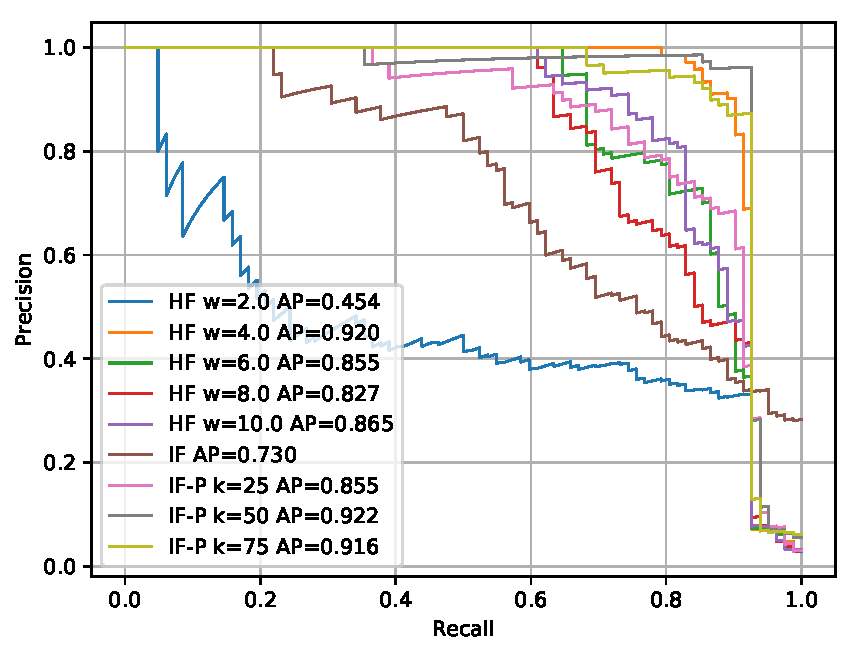
\includegraphics[width=\linewidth]{fig/k25T100_prcurves.pdf}
        \caption{$K=25, T=100$}
    \end{subfigure}
    \hfill
    \begin{subfigure}[t]{0.32\textwidth}
        \centering
        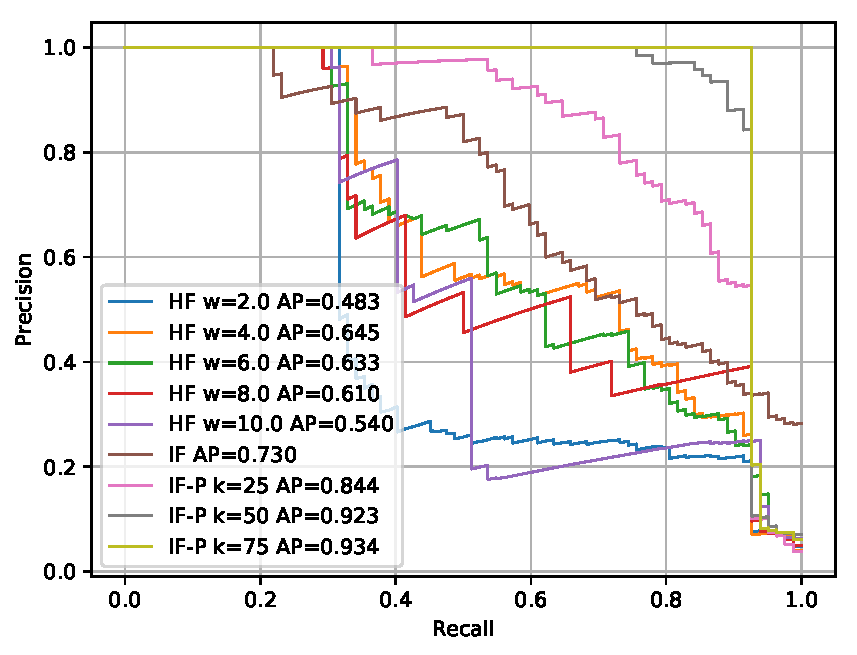
\includegraphics[width=\linewidth]{fig/k50T100_prcurves.pdf}
        \caption{$K=50, T=100$}
    \end{subfigure}
		\hfill
    \begin{subfigure}[t]{0.32\textwidth}
        \centering
        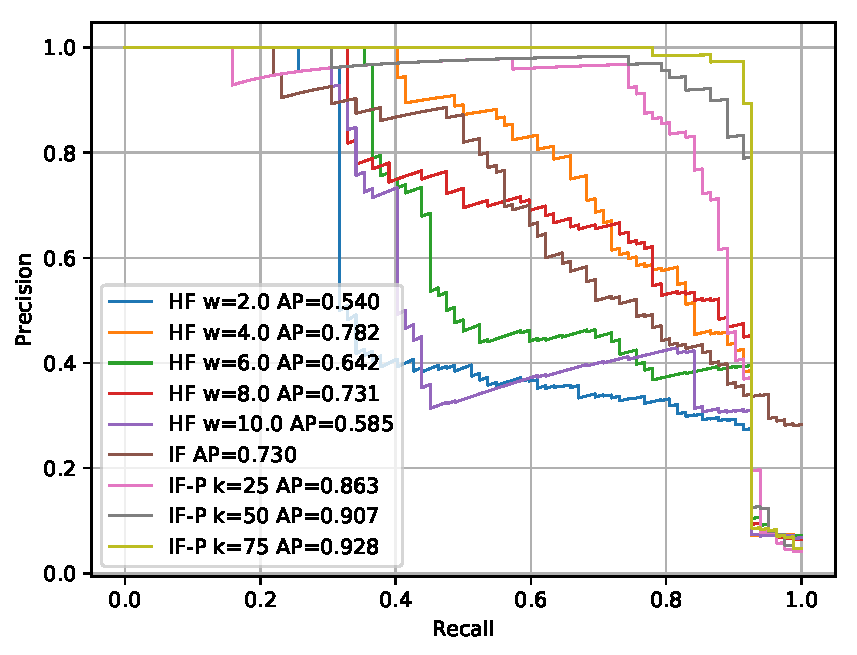
\includegraphics[width=\linewidth]{fig/k50T200_prcurves.pdf}
        \caption{$K=50, T=200$}
    \end{subfigure}
    \caption{Precision-recall curves on synthetic data with 100 noisy dimensions.}
\end{figure*}

Observations from Figure 1:
\begin{enumerate}
	\item HF with $K = 25, T=100, w=4.0$ is on par with iForest with 100 trees on the data projected to $k = 50$ or $k = 75$ dimensions, and better than iForest for $k=25$.

	\item HF with $K = 50, T=100$ has poor performance for all $w$. This was our configuration setting for the previous histogram experiments (with some minor variations): we considered them a failure without trying a \textit{lower} value of $K$. This suggests that $K$ as a measure of data approximation quality may not be the right interpretation.

	\item HF with $K = 50, T=200$ improves performance over $T=100$ slightly, for all $w$.
\end{enumerate}

\subsection{Interpretation --- Approximate Nearest Neighbors}

\begin{wrapfigure}[23]{r}{0.35\textwidth}
    \centering
		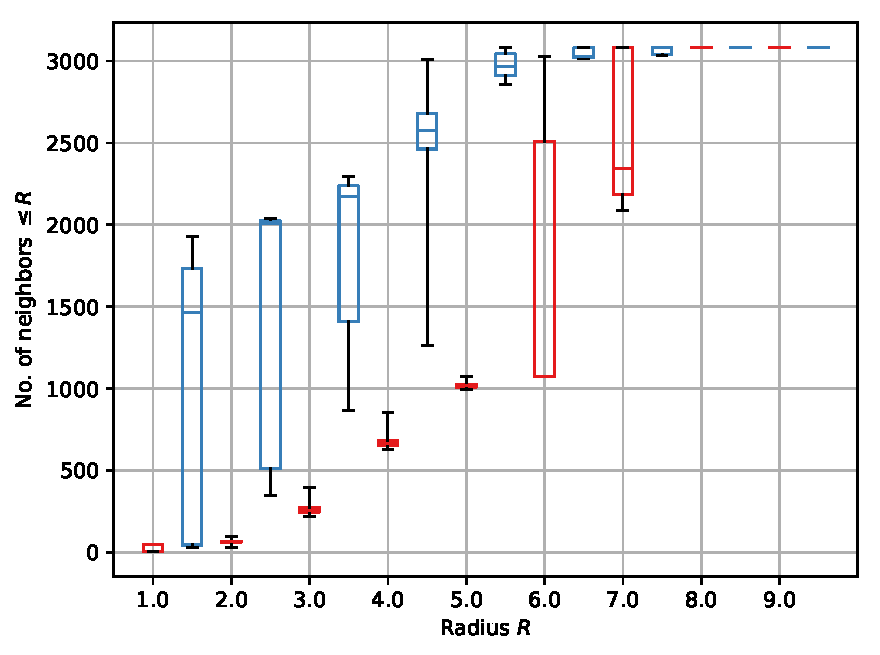
\includegraphics[width=\linewidth]{fig/exact_nn.pdf}
		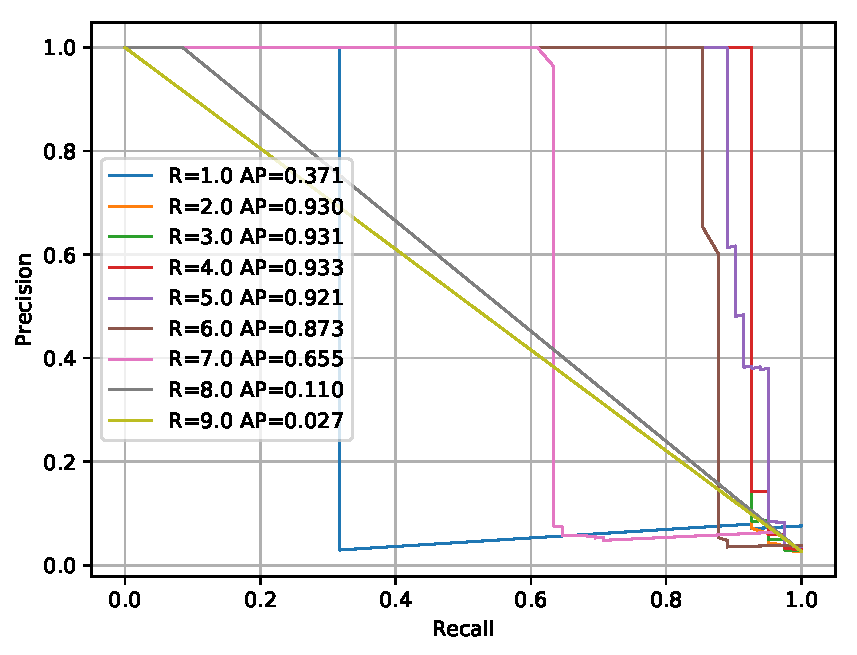
\includegraphics[width=\linewidth]{fig/exact_prcurve.pdf}
    \caption{\small(Top) Number of neighbors within radius $R$, for anomalous (red) and benign (blue) points. (Bottom) PR curves using exact nearest neighbor counts.}
\end{wrapfigure}

The binned data point in our histogram is identical to a point ``hashed'' using 2-stable distributions (\cite{datar2004locality}, 3.1), which extends LSH to solve the approximate nearest neighbors problem in $L_2$. In this method, each point $x$ is ``hashed'' using the function $h(x) = \floor{\frac{x^Ta + b}{w}}$ where $a$ is a random Gaussian vector, $b$ is a random shift and $w$ is the bin width. The probability that two points $x$ and $y$ hash to the same value is proportional to $\|x-y\|_2$.

Each point is hashed $K$ times, and points that agree on all $K$ values are considered candidate nearest neighbors. However, as $K$ grows, it becomes less likely that even nearby points agree on all $K$ values; hence, the process is repeated $T$ times, and the points agreeing on all $K$ values at in least one of the $T$ trials are considered candidate nearest neighbors.

Each configuration of $K, T$ and $w$ results in a certain \textit{probability gap} for points to be considered nearest neighbors. Specifically, this probability gap is defined by the 4-tuple $(R, p_1, cR, p_2)$:
\begin{itemize}
	\item The probability of two points with distance $\leq R$ being hashed to the same values is $\geq p_1$.
	\item The probability of two points with distance $\geq cR$ being hashed to the same values is $\leq p_2$.
\end{itemize}

Hence, our anomaly score for a point can be viewed as the negative of the approximate number of points within a sphere of some radius $R$ centered at that point. The optimal $R$ for anomaly detection on a given dataset is data-dependent (Fig. 2). Hence, the optimal $K, T, w$ are also data-dependent. This explains why a $K=25$ histogram forest may perform better than a $K=50$ one.

\subsection{Data-dependent Parameter Tuning}

\begin{wrapfigure}[14]{r}{0.3\textwidth}
    \centering
		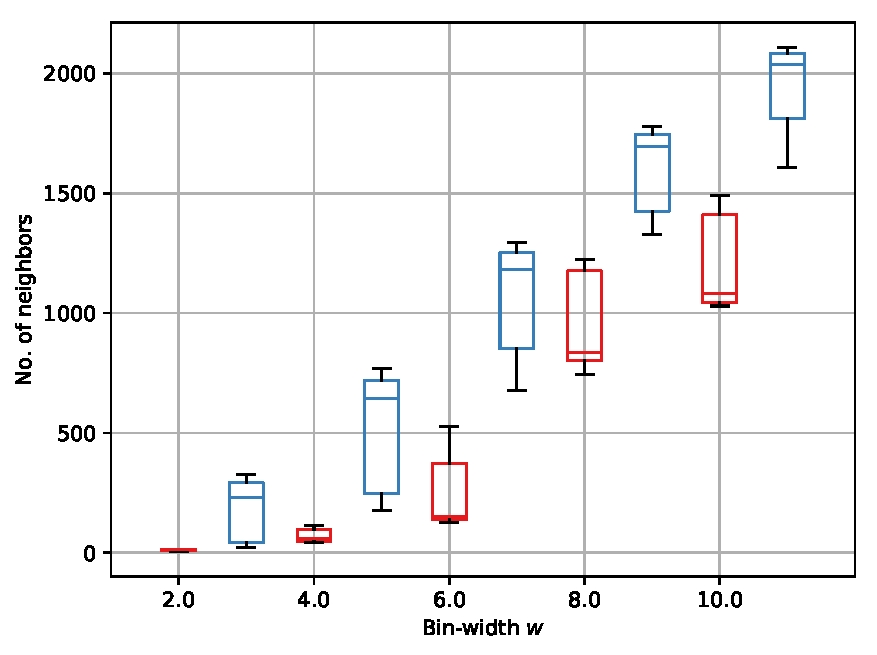
\includegraphics[width=\linewidth]{fig/K25T100_nn.pdf}
		\includegraphics[width=\linewidth]{fig/k25T100_pr2.pdf}
    \caption{\small (Top) Distribution of approximate nearest neighbor counts via HF for different $w$ (Bottom) PR curve for HF. $K=25, T=100$.}
\end{wrapfigure}

The anomaly detection performance is sensitive to picking the right parameters $K, T$ and $w$ (equivalent to picking a radius $R$ and the LSH approximation probabilities $p_1$ and $p_2$). There have been some approaches to auto-tuning the LSH parameters based on the data. However, they were primarily designed for nearest-neighbor search and do not work for data streams. Could we design a data structure for data streams that is tailored for anomaly detection?

\begin{itemize}
	\item LSH-Forest \parencite{bawa2005lsh}. The earliest approach; this is a very simple approache that builds a trie using each bit of the $K$-element sketch. Demonstrated for the Jaccard and cosine distances (since their LSH values are binary). A theoretical analysis was recently published \parencite{andoni2017lsh}.

	\item Parameter-free LSH \parencite{ahle2017parameter}. The most recent approach, designed for Euclidean distances. This builds a ``multi-level LSH'' data structure that tries multiple values of the projection size $K$, and finds the best level for each nearest-neighbor query.
\end{itemize}

\subsection{Relationship to Chains}

\pagebreak

\section{Chains}

\begin{wraptable}{r}{5cm}
	\centering
	\small
	\begin{tabular}{cl}
		\toprule
		\multicolumn{2}{c}{\textbf{Chain Parameters}}\\
		\addlinespace[0.5em]
		$K$ & Dimension of projected data\\
		$C$ & Number of chains\\
		$D$ & Chain depth\\
		$\Delta_f$ & Initial/maximum bin width\\
		\addlinespace[0.5em]
		\multicolumn{2}{c}{\textbf{Other variables}}\\
		\addlinespace[0.5em]
		$f$ & A feature index in $1, \dots, K$\\
		$X$ & $N\times D$ data matrix\\
		$Y$ & $N\times K$ projected data matrix\\
		$A$ & $K\times D$ projection matrix\\
		$b_{if}$ & Shift $\sim \textrm{Uniform}(0,\Delta_f)$\\
		$H_{id}$ & Hashtable/count-min sketch\\
		\bottomrule
	\end{tabular}
	\caption{Notation.}
\end{wraptable}

\textbf{Pre-initialization.} This is done once, and is unchanged for all chains.
\begin{enumerate}
	\item \textbf{Initialize the random projection matrix $A$.}
	\item \textbf{Project the data.} $Y = XA^T$.
	\item \textbf{Set $\Delta_f =$} half the range of projected feature $f$.
	\item \textbf{Sample a shift $b_{if}$} for each chain $i$ and feature $f$.
\end{enumerate}

\textbf{Chain fitting.} For each chain $i = 1, \dots, C$:

\quad For each depth $d = 1, \dots, D$:
\begin{enumerate}
	\item \textbf{Sample a dimension} $f_d \in \{1, \dots K\}$ and store the dimension sampled at each depth. Let $0 \leq c(f,d) \leq d$ be the number of times dimension $f$ has been sampled in the chain until depth $d$.

	\item \textbf{Bin the data.} Let $Y_j = (y_{j1}, \dots, y_{jK})$ be a projected data point. Denote by the $Z_{jd}[f]$ the ``unfloored bin index'' of feature $f$ for point $j$ at depth $d$:
	\begin{eqnarray}
		Z_{jd}[f] = \frac{y_{jf} + b_{if}/2^{c(f,d)-1}}{\Delta_f/2^{c(f,d)-1}}\quad\forall f = 1, \dots K
	\end{eqnarray}
		At depth $d$, the bin indices $\bar{Y}_{jd}$ are logically defined as follows, for $f = 1, \dots, K$:
	\begin{eqnarray}
		\bar{Y}_{jd}[f] =
		\begin{cases}
			 0,\quad\quad\quad\quad~~~\textrm{if } c(f,d) = 0\\
			 \floor{Z_{jd}[f]}\quad\quad\textrm{ if } c(f,d) > 0
		 \end{cases}
	\end{eqnarray}
	In practice, the bins are computed recursively at each depth as follows:
	\begin{eqnarray}
		\bar{Y}_{jd}[f] =
		\begin{cases}
			0\quad\quad\quad\quad\quad\quad\quad\quad\quad~~~~\textrm{ if } c(f,d) = 0\\
			\floor{Z_{jd}[f]}\quad\quad\quad\quad\quad\quad~~~~\textrm{ if } c(f,d) = 1\\
			\floor{2 \times Z_{jd-1}[f] - \frac{b_{if}}{\Delta_f}}\quad\quad\textrm{ if } c(f,d) > 1
		\end{cases}
	\end{eqnarray}
	The recurrence is derived as follows:
	\begin{eqnarray}
		x_k = \frac{y + b/2^{k}}{\Delta/2^k}
			= \frac{y + b/2^{k-1}}{\Delta/2^{k}} - \frac{b/2^{k}}{\Delta/2^{k}}
				= 2\left(\frac{y + b/2^{k-1}}{\Delta/2^{k-1}}\right) - \frac{b}{\Delta} = 2x_{k-1} - \frac{b}{\Delta}
	\end{eqnarray}

	\item \textbf{Store bin counts.} In an exact hashtable or count-min sketch $H_{id}$, increment the count $H_{id}(\bar{Y}_j)$ for $j = 1, \dots, N$.
\end{enumerate}

\textbf{Scoring at depth $d$.} The anomaly score of a point $X_j$ at depth $d$ is $-\textrm{average}_i(H_{id}(\bar{Y}_j))$.

\pagebreak

\subsection{Results with bin-counts as anomaly scores}

\begin{figure*}[h!]
    \centering
    \begin{subfigure}[t]{0.24\textwidth}
        \centering
        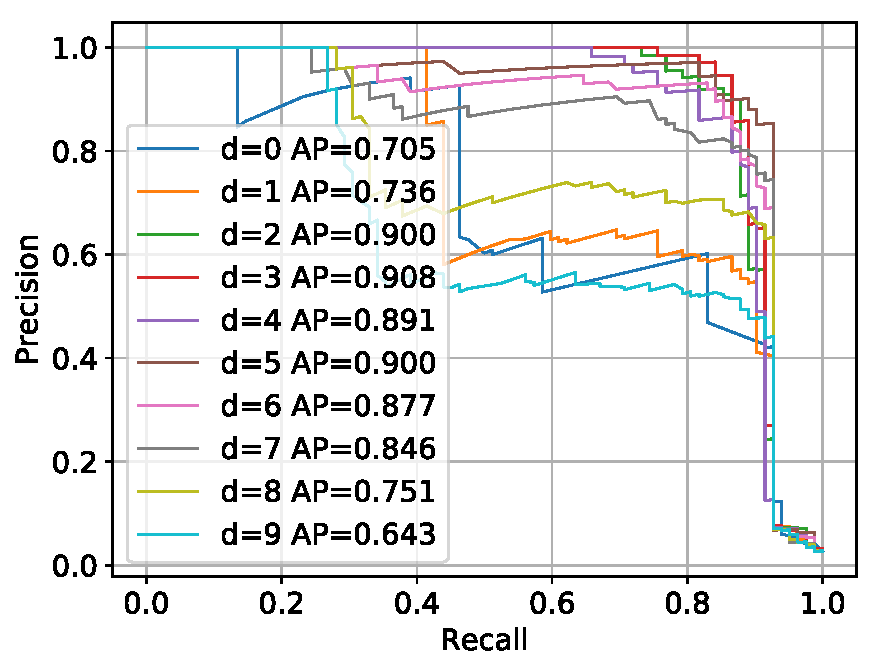
\includegraphics[width=\linewidth]{fig/chains_pr_k50c10d10.pdf}
        \caption{$K=50, C=10$}
    \end{subfigure}
    \hfill
    \begin{subfigure}[t]{0.24\textwidth}
        \centering
        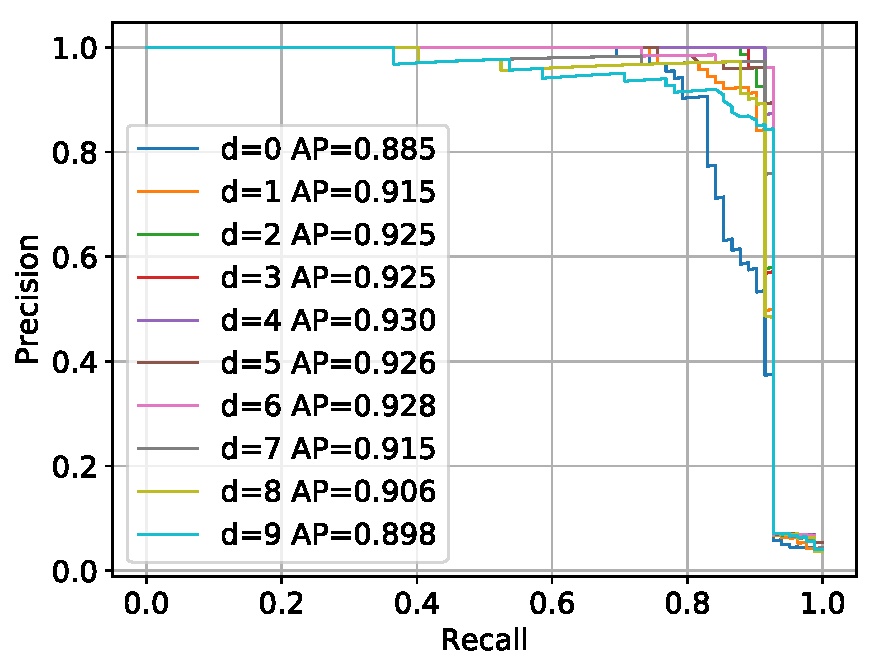
\includegraphics[width=\linewidth]{fig/chains_pr_k50c50d10.pdf}
        \caption{$K=50, C=50$}
    \end{subfigure}
		\hfill
    \begin{subfigure}[t]{0.24\textwidth}
        \centering
        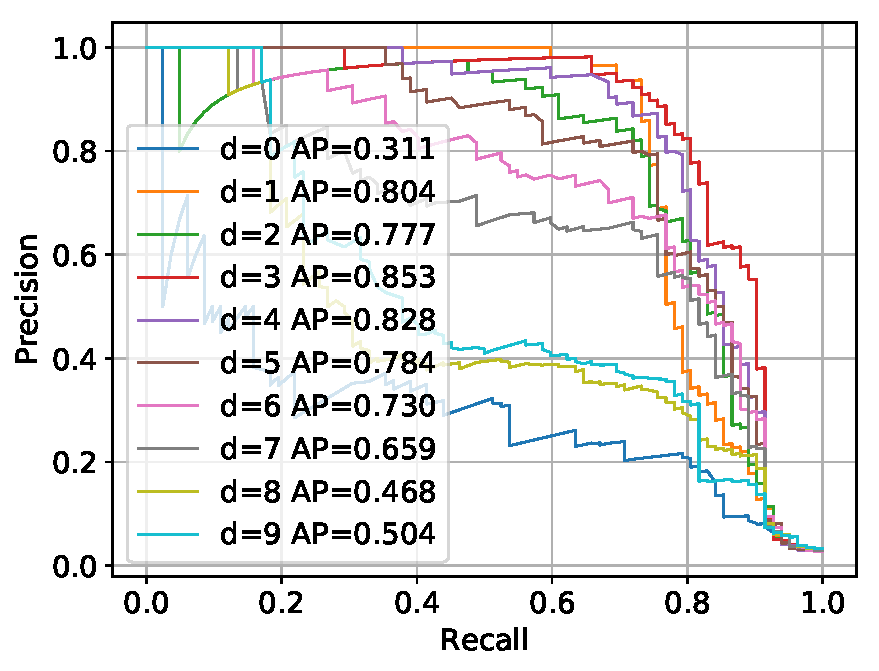
\includegraphics[width=\linewidth]{fig/chains_pr_k25c10d10.pdf}
        \caption{$K=25, C=10$}
    \end{subfigure}
		\hfill
    \begin{subfigure}[t]{0.24\textwidth}
        \centering
        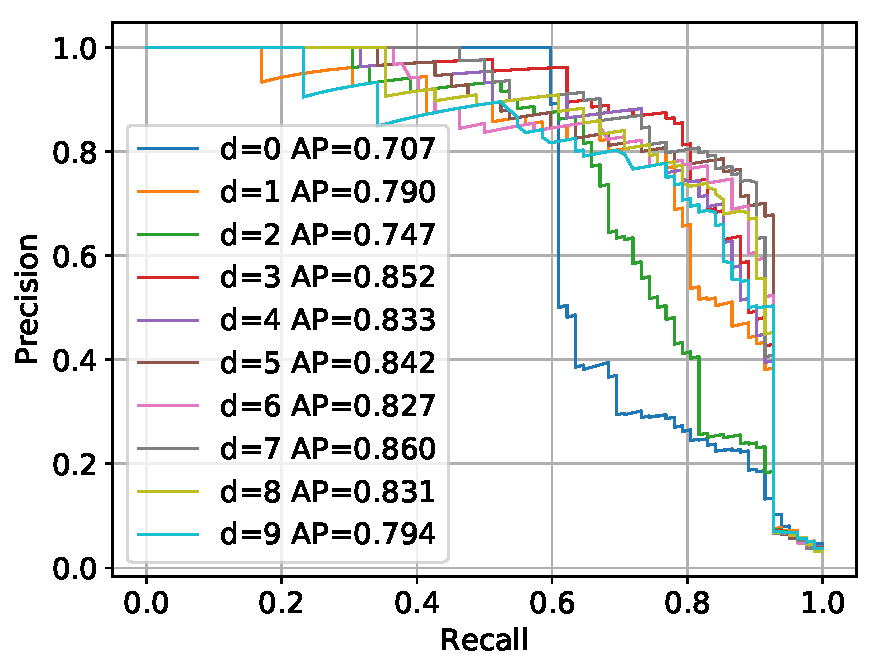
\includegraphics[width=\linewidth]{fig/chains_pr_k25c50d10.pdf}
        \caption{$K=25, C=50$}
    \end{subfigure}
    \caption{Precision-recall curves on synthetic data with 100 noisy dimensions, $D=10$.}
\end{figure*}

\begin{figure*}[h!]
    \centering
    \begin{subfigure}[t]{0.24\textwidth}
        \centering
        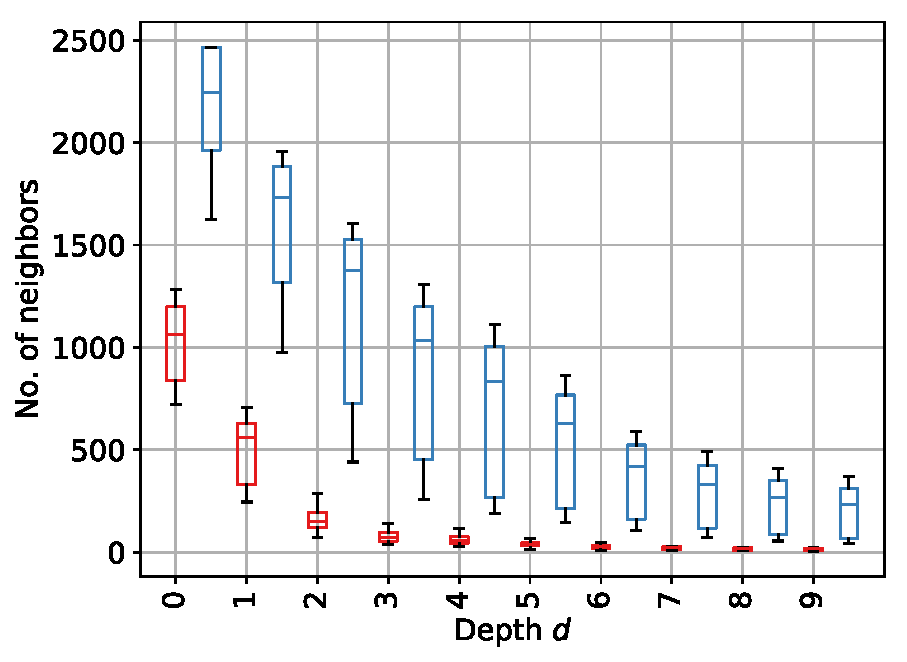
\includegraphics[width=\linewidth]{fig/chains_hist_k50c10d10.pdf}
        \caption{$K=50, C=10$}
    \end{subfigure}
    \hfill
    \begin{subfigure}[t]{0.24\textwidth}
        \centering
        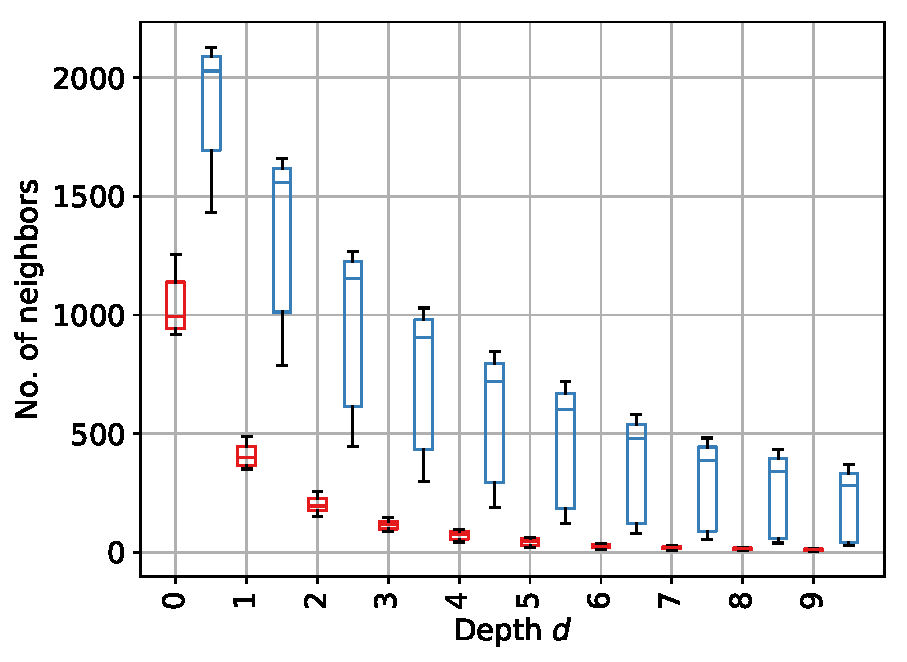
\includegraphics[width=\linewidth]{fig/chains_hist_k50c50d10.pdf}
        \caption{$K=50, C=50$}
    \end{subfigure}
		\hfill
    \begin{subfigure}[t]{0.24\textwidth}
        \centering
        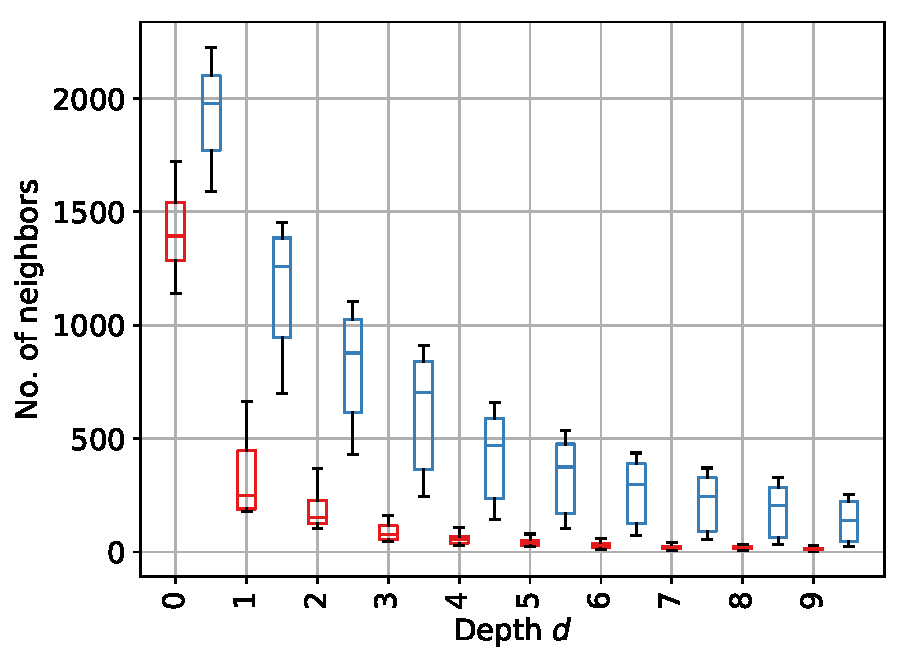
\includegraphics[width=\linewidth]{fig/chains_hist_k25c10d10.pdf}
        \caption{$K=25, C=10$}
    \end{subfigure}
		\hfill
    \begin{subfigure}[t]{0.24\textwidth}
        \centering
        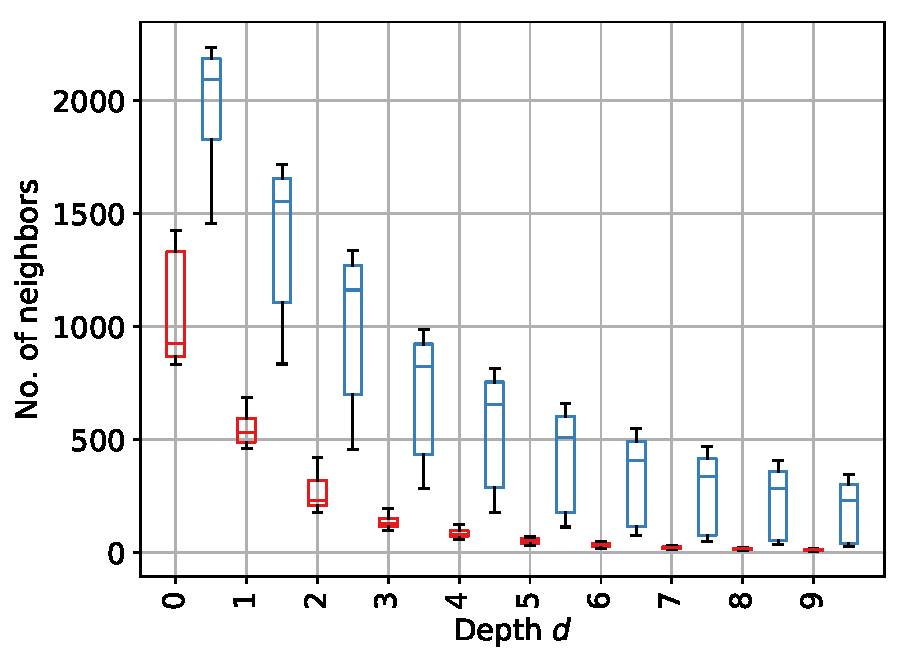
\includegraphics[width=\linewidth]{fig/chains_hist_k25c50d10.pdf}
        \caption{$K=25, C=50$}
    \end{subfigure}
    \caption{No. of neighbors in the same bin for anomalous (red) and benign (blue) points.}
\end{figure*}

\subsection{Results with LOCI scores as anomaly scores}

Previously, we scored each point $X_j$ using chain $i$ at depth $d$ using the number of neighbors lying in the same bin, $H_{id}(\bar{Y}_j)$. We modify this to obtain a LOCI score $L_{id}(\bar{Y}_j)$ as:
\begin{eqnarray}
	\bar{H}_{id}(\bar{Y}_j) &=& H_{id}(\bar{Y}_j) \times 2^d\\
	L_{id}(\bar{Y}_j) &=& \bar{H}_{id}(\bar{Y}_j) - \frac{1}{N-1}\sum_{k \neq j}\bar{H}_{id}(\bar{Y}_k)
\end{eqnarray}
Then the anomaly score of a point $X_j$ is $-\textrm{average}_i\left(\textrm{min}_d L_{id}(\bar{Y}_j)\right)$.

\begin{figure*}[ht!]
    \centering
    \begin{subfigure}[t]{0.24\textwidth}
        \centering
        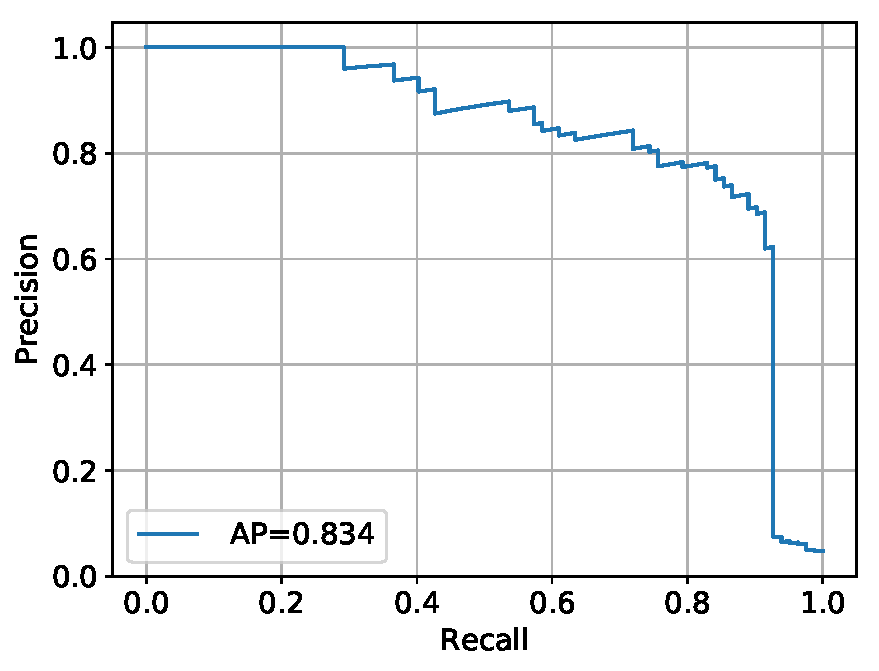
\includegraphics[width=\linewidth]{fig/chains_anomalyscore_pr_k50c10d10.pdf}
        \caption{$K=50, C=10$}
    \end{subfigure}
    \hfill
    \begin{subfigure}[t]{0.24\textwidth}
        \centering
        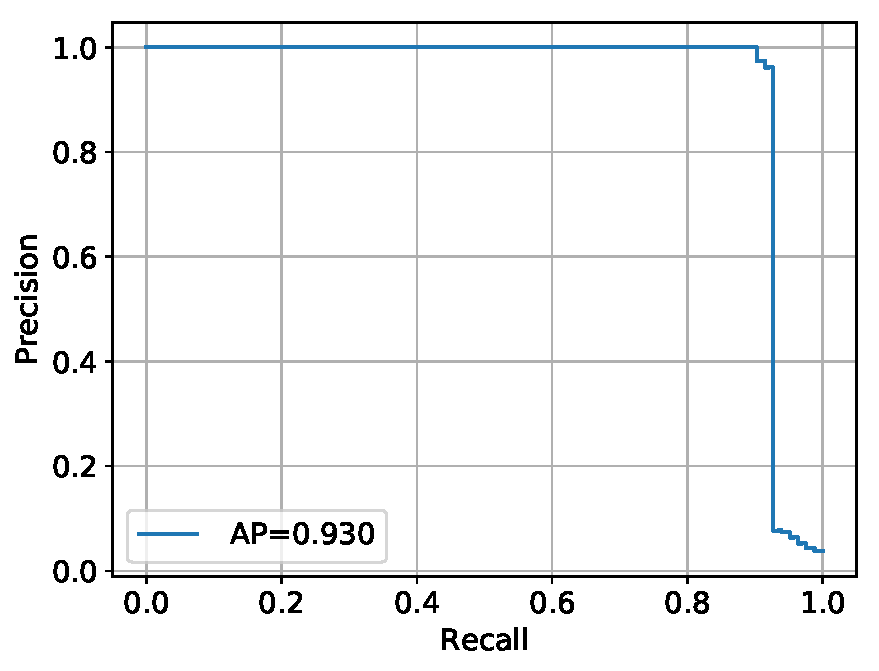
\includegraphics[width=\linewidth]{fig/chains_anomalyscore_pr_k50c50d10.pdf}
        \caption{$K=50, C=50$}
    \end{subfigure}
		\hfill
    \begin{subfigure}[t]{0.24\textwidth}
        \centering
        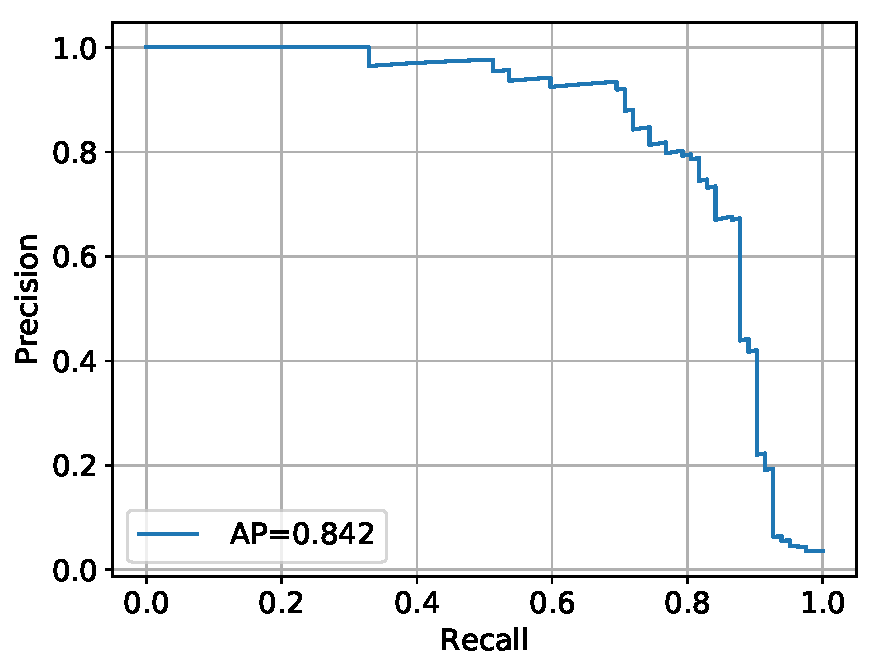
\includegraphics[width=\linewidth]{fig/chains_anomalyscore_pr_k25c10d10.pdf}
        \caption{$K=25, C=10$}
    \end{subfigure}
		\hfill
    \begin{subfigure}[t]{0.24\textwidth}
        \centering
        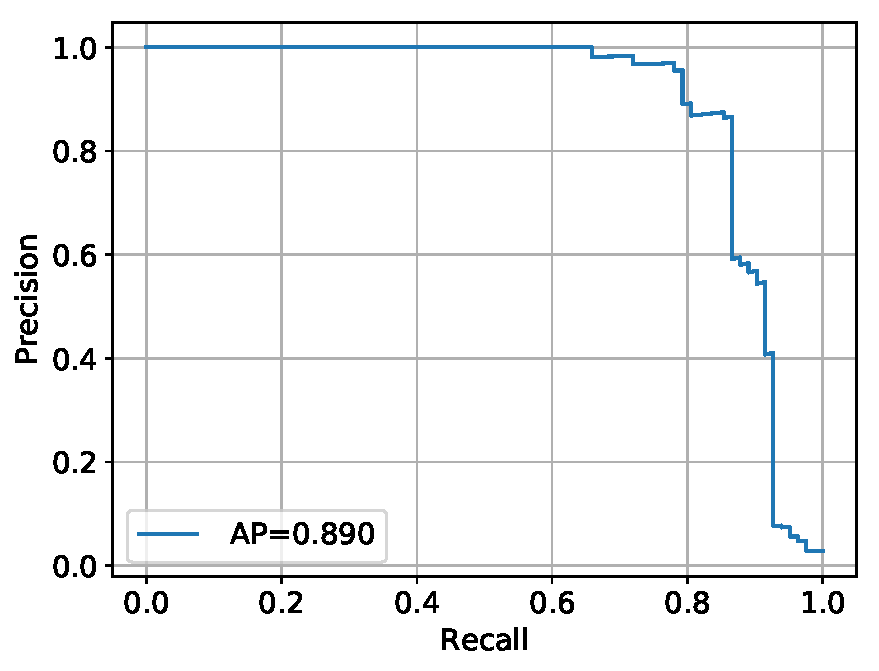
\includegraphics[width=\linewidth]{fig/chains_anomalyscore_pr_k25c50d10.pdf}
        \caption{$K=25, C=50$}
    \end{subfigure}
    \caption{Precision-recall curves on synthetic data with 100 noisy dimensions, $D=10$.}
\end{figure*}

\begin{figure*}[ht!]
    \centering
    \begin{subfigure}[t]{0.24\textwidth}
        \centering
        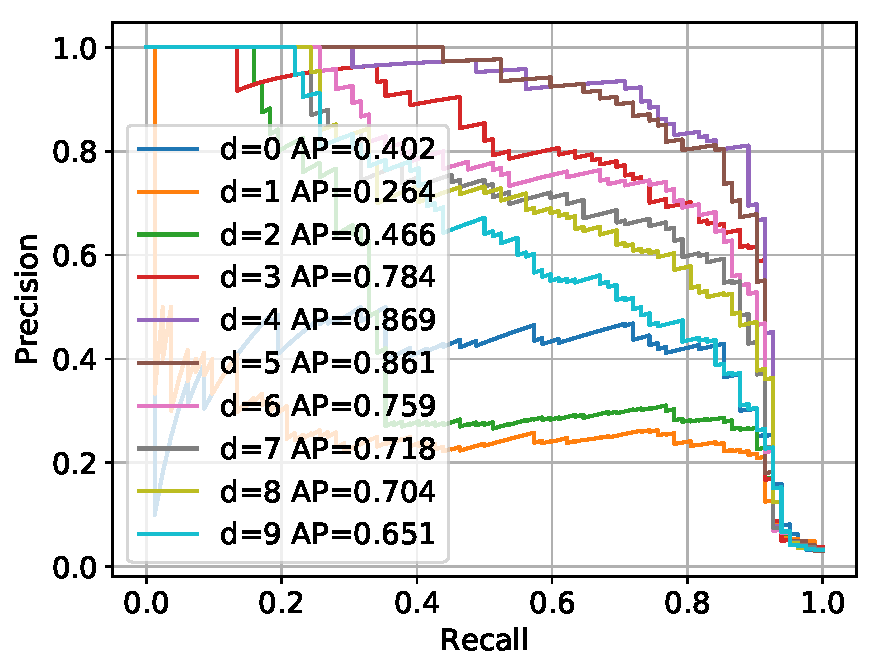
\includegraphics[width=\linewidth]{fig/chains_lociscore_pr_k50c10d10.pdf}
        \caption{$K=50, C=10$}
    \end{subfigure}
    \hfill
    \begin{subfigure}[t]{0.24\textwidth}
        \centering
        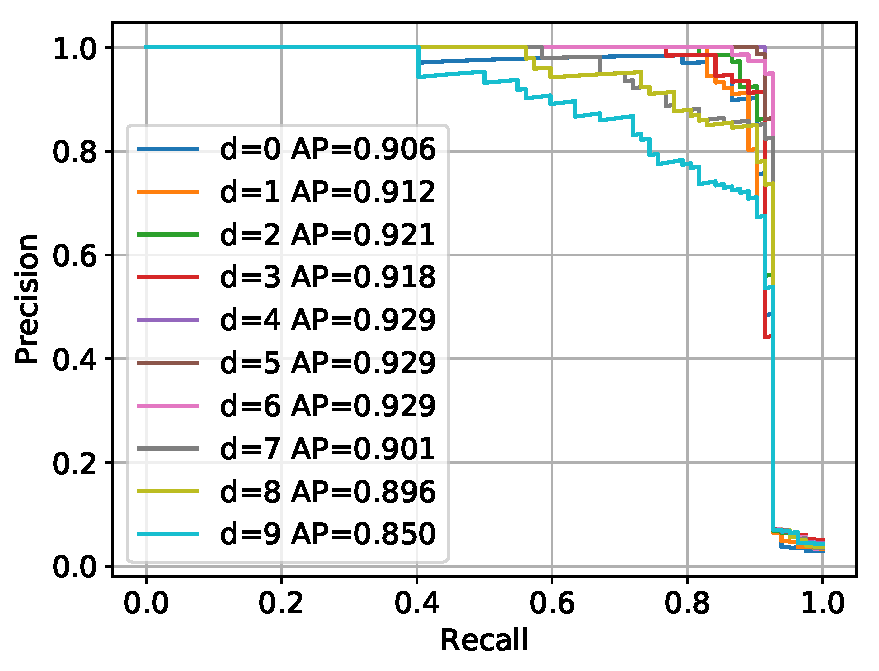
\includegraphics[width=\linewidth]{fig/chains_lociscore_pr_k50c50d10.pdf}
        \caption{$K=50, C=50$}
    \end{subfigure}
		\hfill
    \begin{subfigure}[t]{0.24\textwidth}
        \centering
        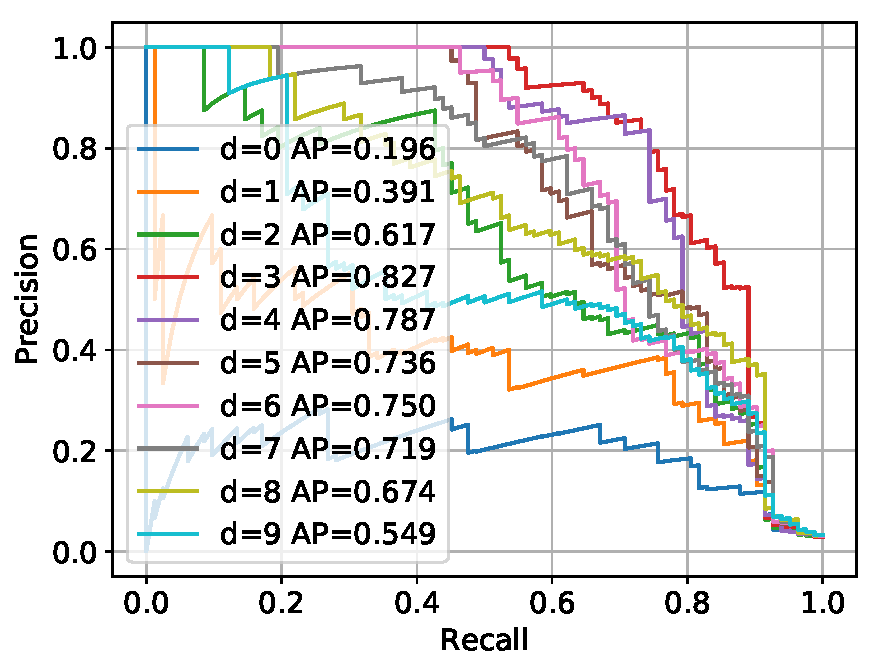
\includegraphics[width=\linewidth]{fig/chains_lociscore_pr_k25c10d10.pdf}
        \caption{$K=25, C=10$}
    \end{subfigure}
		\hfill
    \begin{subfigure}[t]{0.24\textwidth}
        \centering
        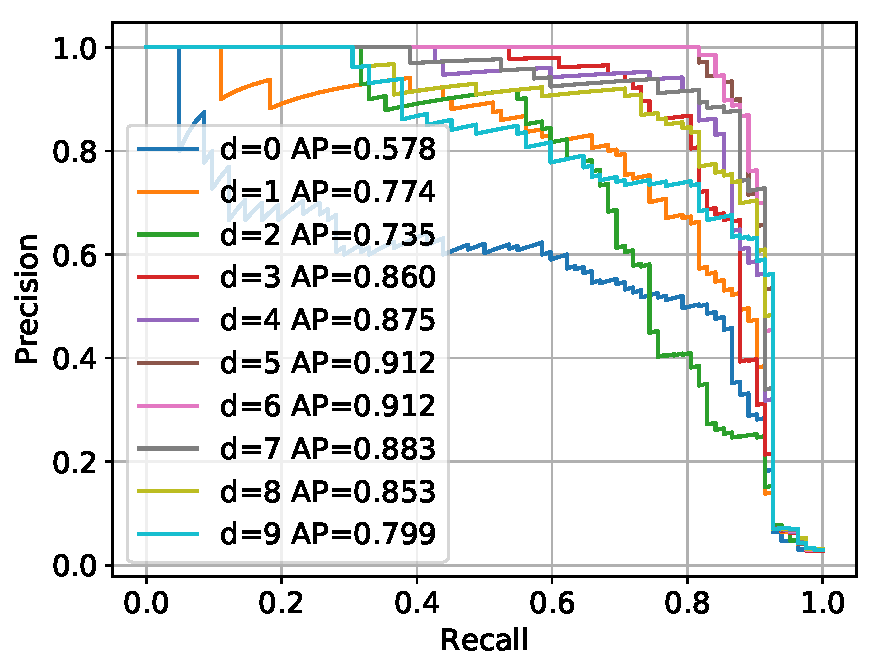
\includegraphics[width=\linewidth]{fig/chains_lociscore_pr_k25c50d10.pdf}
        \caption{$K=25, C=50$}
    \end{subfigure}
    \caption{Precision-recall curves with LOCI scores at different depths $d$.}
\end{figure*}

\pagebreak

\subsection{Stability across runs}

\begin{table}[ht!]
    \centering
		\begin{tabular}{lll}
				\toprule
				\textbf{Chain Parameters} & \textbf{Mean AP} & \textbf{Standard Deviation}\\
				\midrule
				$K=50, C=10$ & 0.824 & 0.064\\
				$K=50, C=50$ & 0.930 & 0.001\\
				$K=25, C=10$ & 0.742 & 0.123\\
				$K=25, C=50$ & 0.901 & 0.019\\
				\bottomrule
		\end{tabular}
		\caption{Chain AP stability across 5 runs, $D=10$.}
\end{table}

\subsection{Number of unique bin IDs with depth}

\begin{figure}[h!]
	\centering
	\begin{subfigure}[b]{0.3\textwidth}
			\centering
			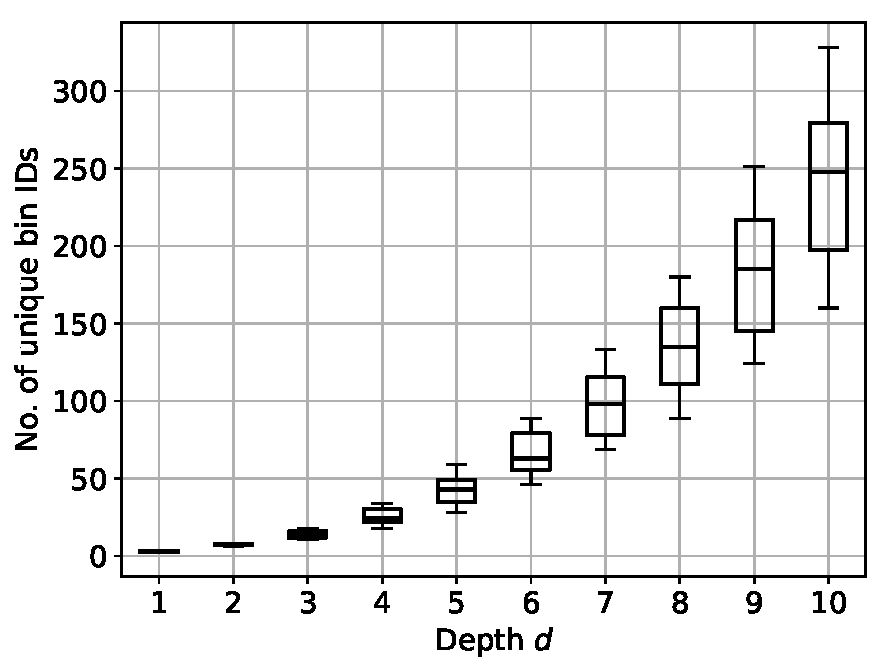
\includegraphics[width=\linewidth]{fig/chains_binids_k50c100d10.pdf}
	\end{subfigure}
	\caption{No. of unique bins for $C=100$ chains, $K=50, d=10$.}
\end{figure}

\subsection{Scores for different anomaly types}

Fig. 9 illustrates how the anomaly scores vary for different classes of points, shown in Fig. 9(a):
\begin{table}[h!]
	\centering
	\begin{tabular}{llll}
		\toprule
		\textbf{Class} & \textbf{No. of points} & \textbf{Description} & \textbf{Color}\\
		\midrule
		Class 0 & 1000 & Benign sparse points & Blue\\
		Class 1 & 2000 & Benign dense points & Orange\\
		Class 2 & 50 & Anomalous dense points & Green\\
		Class 3 & 25 & Anomalous sparse points & Red\\
		Class 4 & 6 & Locally anomalous points & Purple\\
		Class 5 & 1 & Single anomalous point & Brown\\
		\bottomrule
	\end{tabular}
\end{table}

\pagebreak

From Fig. 9(b) conforms to intuition: as the depth in the chain increases, the average number of points lying in the same bin (across chains) decreases for all classes of points. This is due to two factors: (i) increasing the number of bin dimensions, and (ii) decreasing the bin width. Point classes lying in denser regions have higher bin counts.

Fig. 9(c) shows the LOCI scores (eq. 6) at each depth $d$, scaled up by $2^d$ for visual clarity. The LOCI score of a point is simply its bin count minus the mean bin count of all other points at that depth. Hence, as $d$ increases and the bin counts of all points tend to 1, the LOCI score tends to 1.

Fig. 9(d) shows the anomaly scores. The order of anomalousness across point classes is inversely proportional to their global density. %Fig. 10 replicates Fig. 9(d) for LODA by fixing $K = 100$ (the number of projections) and varying the bin-width. The optimal bin-width (as determined by LODA) is marked in black.

\begin{figure*}[ht!]
    \centering
    \begin{subfigure}[t]{0.48\textwidth}
        \centering
        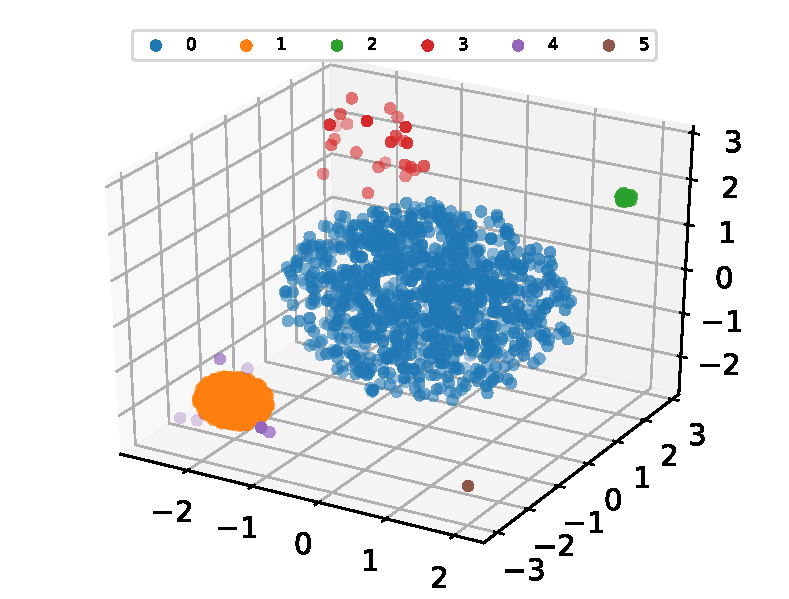
\includegraphics[width=\linewidth]{fig/syndata.pdf}
        \caption{Synthetic data, colored by point class}
    \end{subfigure}
    \hfill
    \begin{subfigure}[t]{0.48\textwidth}
        \centering
        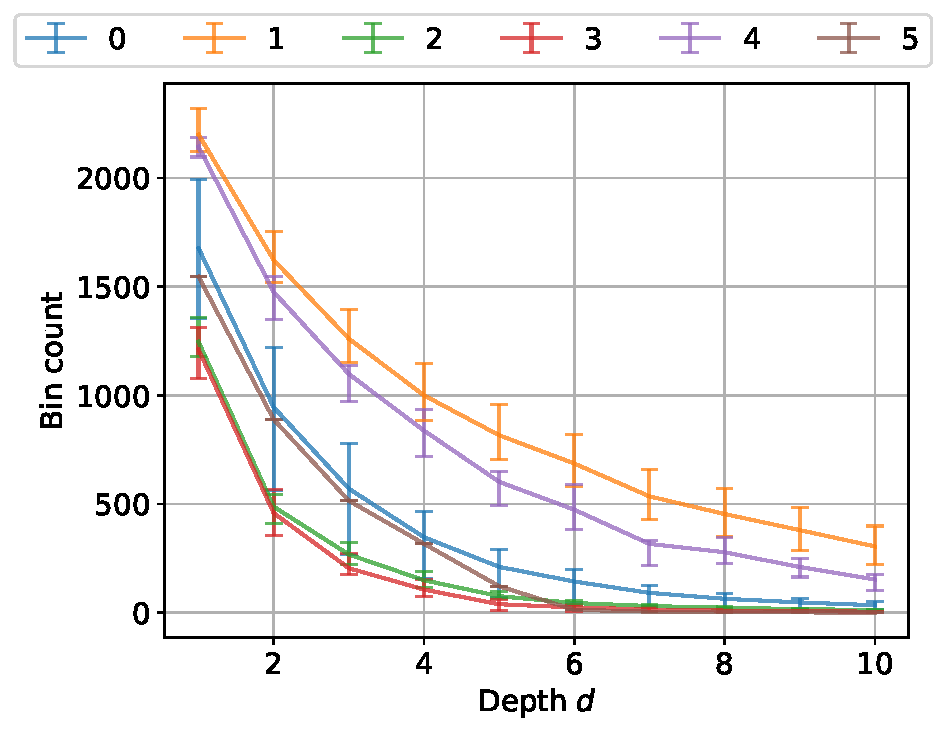
\includegraphics[width=\linewidth]{fig/chains_type_bincounts_k50c50d10.pdf}
        \caption{Bin-counts}
    \end{subfigure}
		\\
    \begin{subfigure}[t]{0.48\textwidth}
        \centering
        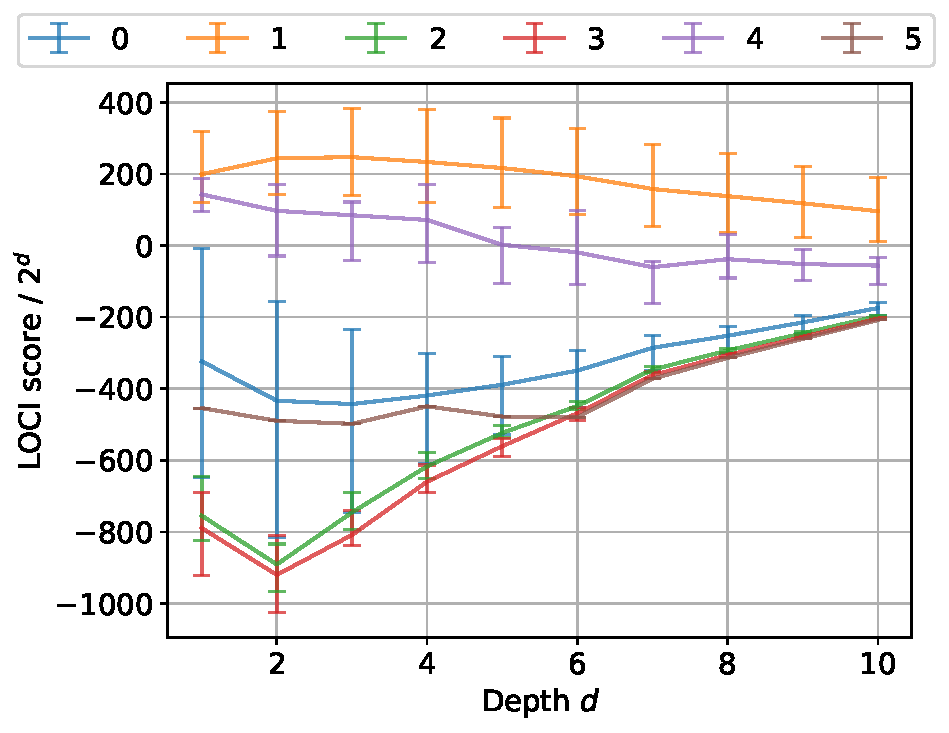
\includegraphics[width=\linewidth]{fig/chains_type_lociscores_k50c50d10.pdf}
        \caption{LOCI scores (mean-adjusted bin-counts)}
    \end{subfigure}
		\hfill
    \begin{subfigure}[t]{0.48\textwidth}
        \centering
        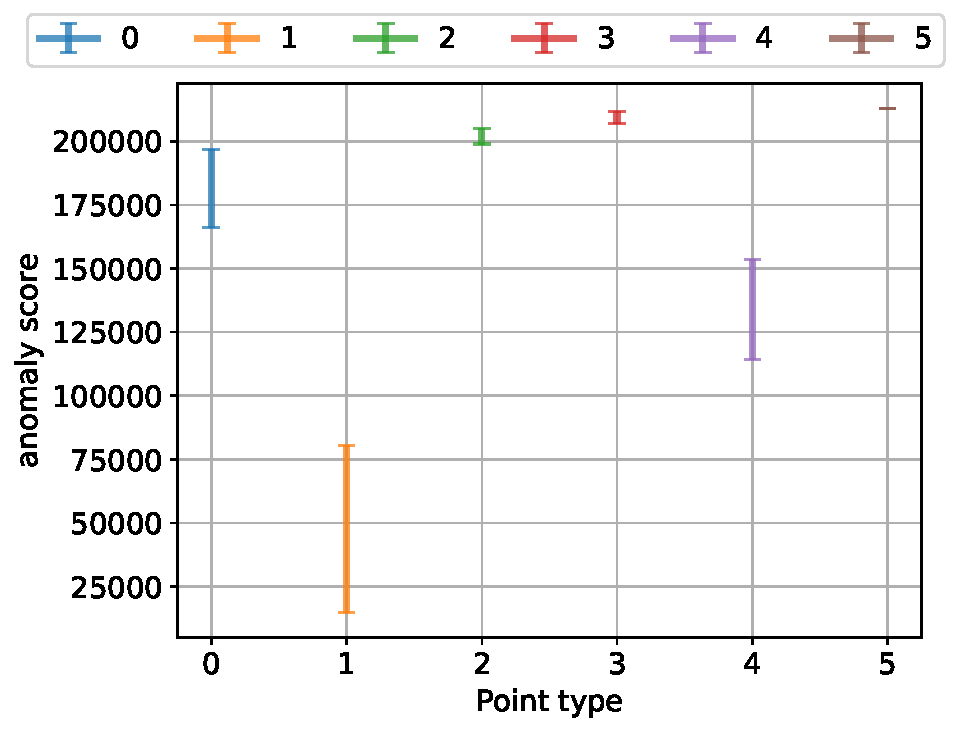
\includegraphics[width=\linewidth]{fig/chains_type_anomscores_k50c50d10.pdf}
        \caption{Anomaly scores (negative of the minimum LOCI score across all depths)}
    \end{subfigure}
    \caption{Score distributions for different point classes (see \S2.3 for details). Error bars indicate the median, 5$^{\textrm{th}}$ and 95$^{\textrm{th}}$ percentile scores across all points. Chains with $K=50, C=100, d=10$.}
\end{figure*}

% \begin{figure*}[ht!]
%     \centering
%     \begin{subfigure}[t]{0.30\textwidth}
%         \centering
%         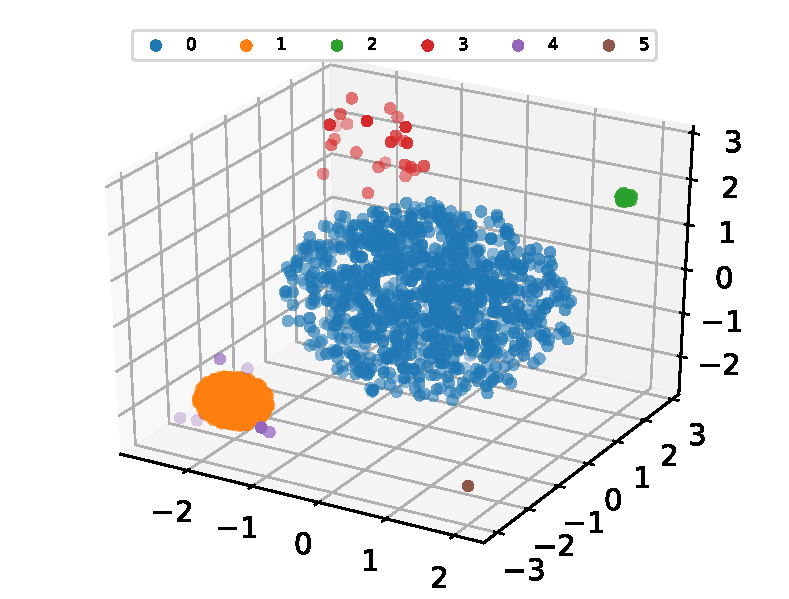
\includegraphics[width=\linewidth]{fig/syndata.pdf}
%         \caption{Synthetic data, colored by point class}
%     \end{subfigure}
%     \hfill
%     \begin{subfigure}[t]{0.30\textwidth}
%         \centering
%         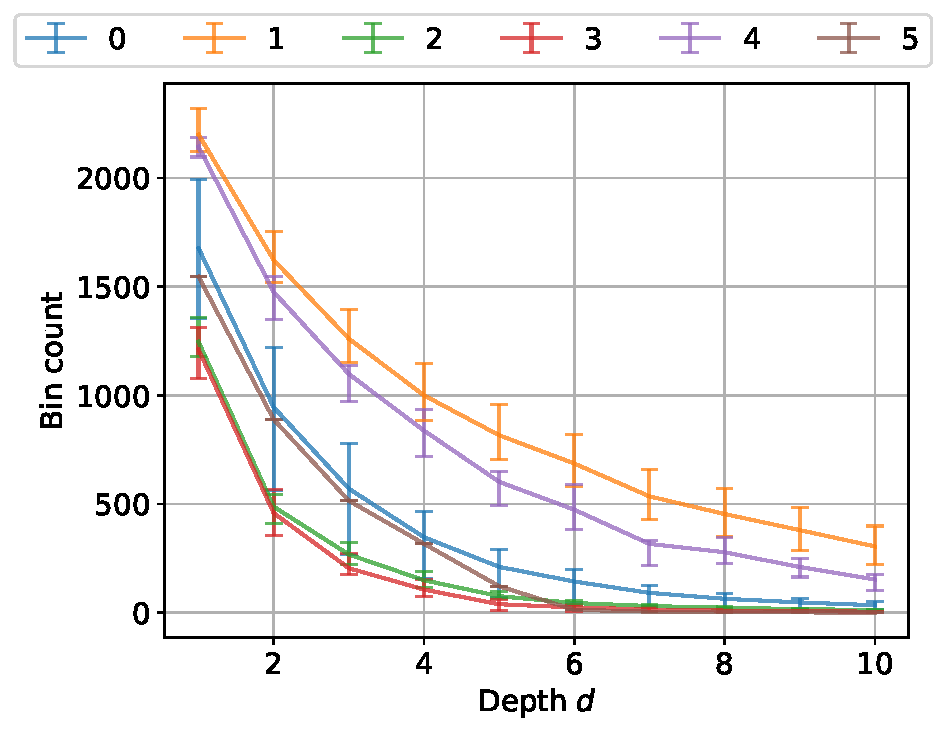
\includegraphics[width=\linewidth]{fig/chains_type_bincounts_k50c50d10.pdf}
%         \caption{Bin-counts}
%     \end{subfigure}
% 		\hfill
% 		\begin{subfigure}[t]{0.30\textwidth}
% 				\centering
% 				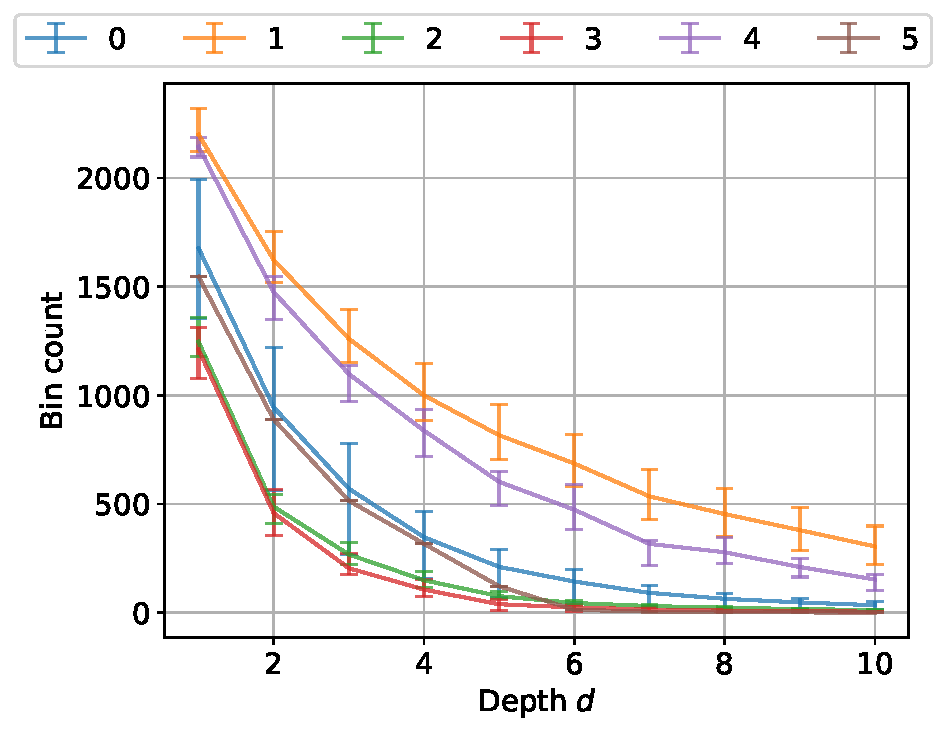
\includegraphics[width=\linewidth]{fig/chains_type_bincounts_k50c50d10.pdf}
% 				\caption{Bin-counts}
% 		\end{subfigure}
%     \caption{Score distributions for different point classes (see \S2.3 for details). Error bars indicate the median, 5$^{\textrm{th}}$ and 95$^{\textrm{th}}$ percentile scores across all points. Chains with $K=50, C=100, d=10$.}
% \end{figure*}

\pagebreak
\subsection{Streaming random projections}

Let the data dimensionality be $D$ and projection dimensionality be $K$. Given a density $s$, the very sparse random projections method \parencite{li2006very} generates $K$ $D$-dimensional vectors containing elements $r_{km}$ as follows ($k = 1, \dots, K, m = 1, \dots, D$):
\begin{eqnarray}
	r_{km} = \begin{cases}
		-\frac{1}{\sqrt{Ks}}\quad\textrm{ with probability }\frac{s}{2}\nonumber\\
		0\quad\textrm{ with probability }1 - s\nonumber\\
		\frac{1}{\sqrt{Ks}}\quad\textrm{ with probability }\frac{s}{2}\\
	\end{cases}
	\label{eq:randomprojections}
\end{eqnarray}
Instead of storing these vectors, we store $K$ hash functions. Each hash function $h_k$ hashes a string $w_m$ (the feature name) to a hash value $h_k(w_m)$, which serves as a plug-in replacement for $r_{km}$ without explicitly storing the random vectors.

The implementation of $h_k$ ensures that the hash values follow the probability distribution prescribed above.

The function $h_k(w_m)$ is implemented as follows:
\begin{enumerate}
	\item $b = g_k(w_m)$, where $g_k$ is drawn from a universal family and $b$ is a 32-bit integer. Having more bits in $b$ provides a more precise approximation to the desired probability distribution, but we found 32 to be sufficient.
	\item $n = b/(2^{32}-1)$ is a number between 0 and 1. With a good universal family to generate $g_k$, $n$ follows distributions $P_{g_k}(n) \sim \textrm{Uniform}(0,1)$ and $P_{w_m}(n) \sim \textrm{Uniform}(0,1)$.
	\item $n$ is used to return a number in $\{\frac{1}{\sqrt{Ks}}, 0, \frac{1}{\sqrt{Ks}}\}$ with the desired probability distribution:
		\begin{enumerate}
			\item If $0 \leq n < s/2$, return $-\frac{1}{\sqrt{Ks}}$.
			\item If $s/2 \leq n < s$, return $\frac{1}{\sqrt{Ks}}$.
			\item If $s \leq n \leq 1$, return 0.
		\end{enumerate}
\end{enumerate}

It is very important that $g_k$ be drawn from a universal (or almost-universal) string hash family with good empirical randomization properties. SipHash \parencite{aumasson2012siphash} and MurmurHash3\footnote{\url{https://github.com/aappleby/smhasher/blob/master/src/MurmurHash3.cpp}} were found to perform well, whereas multiplicative hashing does not.

Fig. \ref{fig:distortion} illustrates the empirical distortion of this streaming random projection method on the synthetic data, for both the Euclidean and cosine distances. Fig. \ref{fig:distortion-static} illustrates the distortion using the standard, static random projections.

When used as a plug-in replacement for sparse random projections in XStream on the synthetic data, there was no significant drop in average precision (mean and standard deviation reported for 5 runs): AP = $0.823 \pm 0.088$ for $K = 50, C = 50$; AP = $0.916 \pm 0.009$ for $K = 100, C = 50$; AP = $0.927 \pm 0.003$ for $K = 100, C = 100$.

\begin{figure*}[h!]
    \centering
    \begin{subfigure}[t]{0.29\textwidth}
        \centering
        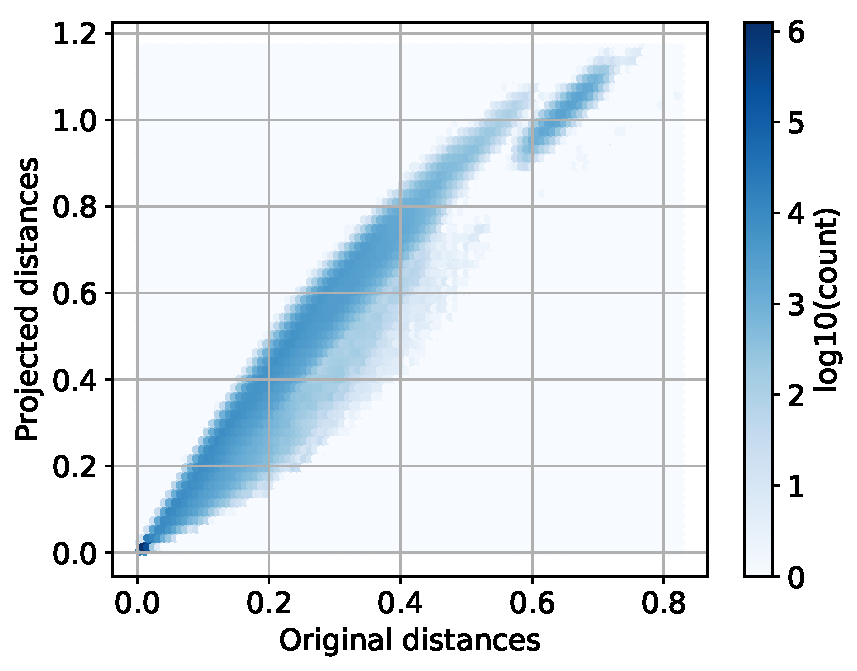
\includegraphics[width=\linewidth]{fig/streamhash_projection_cosine_k50.pdf}
        \caption{$K=50$, cosine.}
    \end{subfigure}
    \hfill
		\begin{subfigure}[t]{0.29\textwidth}
				\centering
				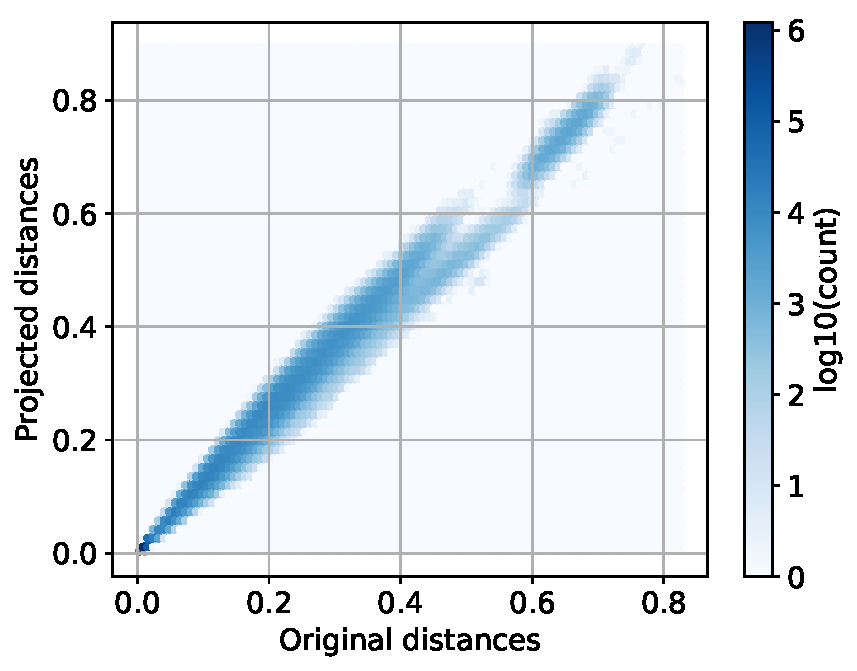
\includegraphics[width=\linewidth]{fig/streamhash_projection_cosine_k100.pdf}
				\caption{$K=100$, cosine.}
		\end{subfigure}
		\hfill
		\begin{subfigure}[t]{0.29\textwidth}
				\centering
				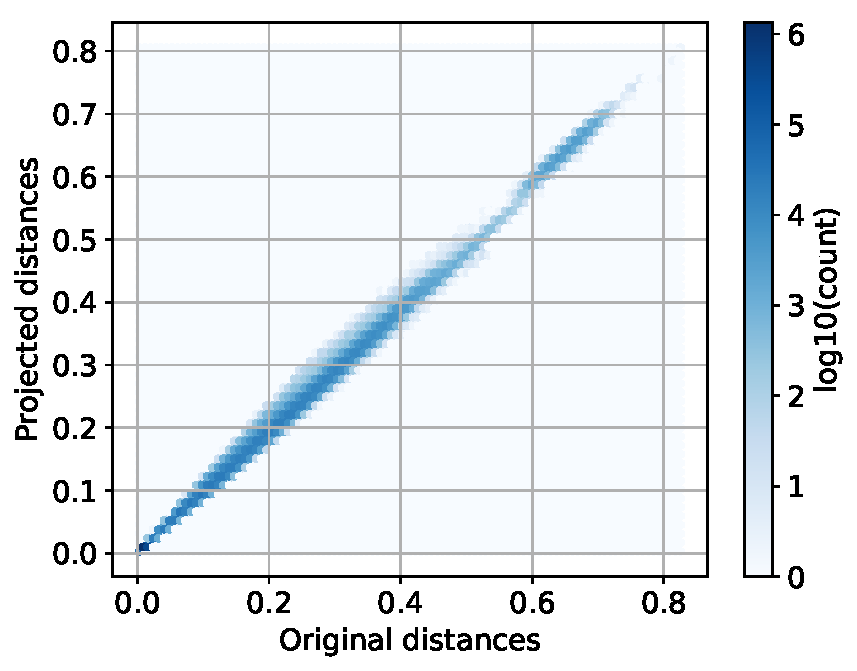
\includegraphics[width=\linewidth]{fig/streamhash_projection_cosine_k1000.pdf}
				\caption{$K=1000$, cosine.}
		\end{subfigure}\\
		\begin{subfigure}[t]{0.29\textwidth}
				\centering
				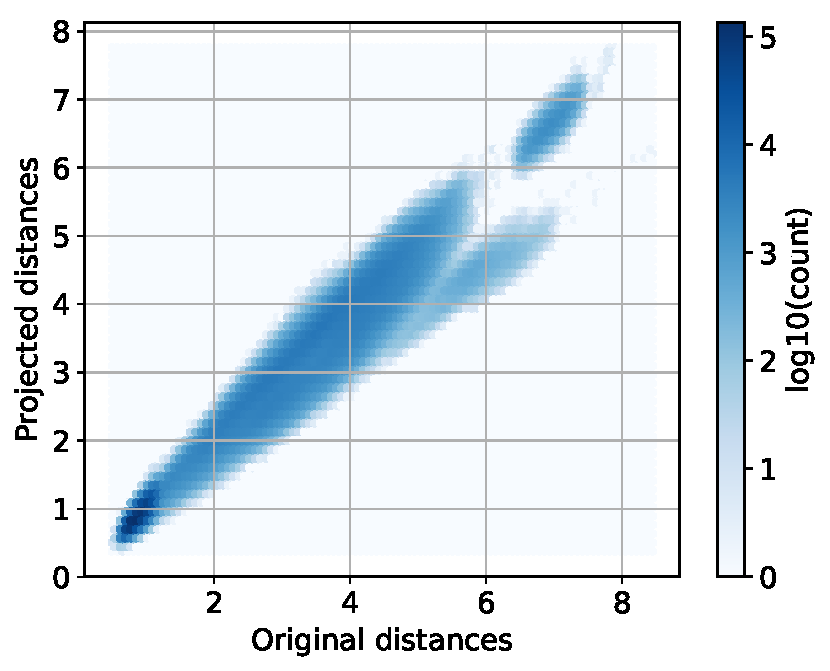
\includegraphics[width=\linewidth]{fig/streamhash_projection_euclidean_k50.pdf}
				\caption{$K=50$, Euclidean.}
		\end{subfigure}
		\hfill
		\begin{subfigure}[t]{0.29\textwidth}
				\centering
				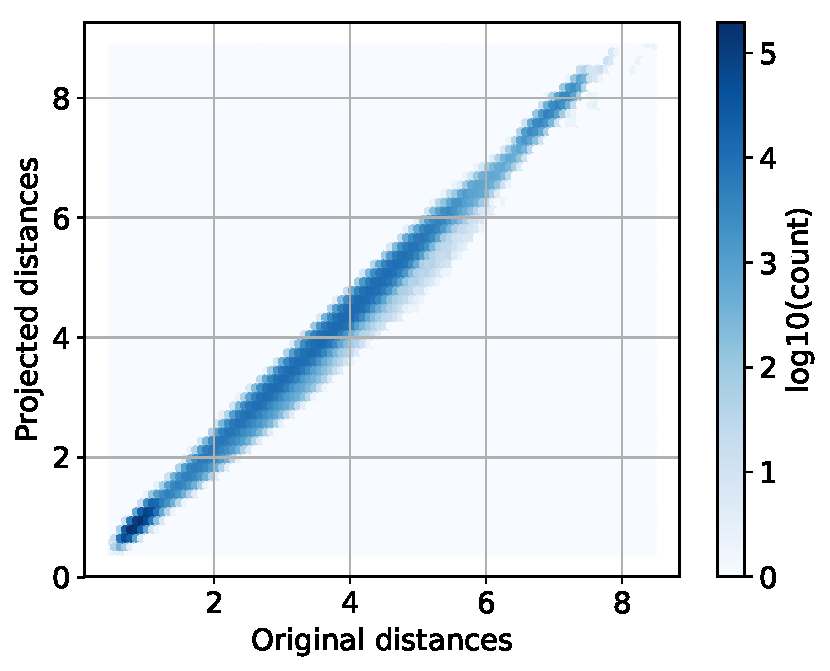
\includegraphics[width=\linewidth]{fig/streamhash_projection_euclidean_k100.pdf}
				\caption{$K=100$, Euclidean.}
		\end{subfigure}
		\hfill
		\begin{subfigure}[t]{0.29\textwidth}
				\centering
				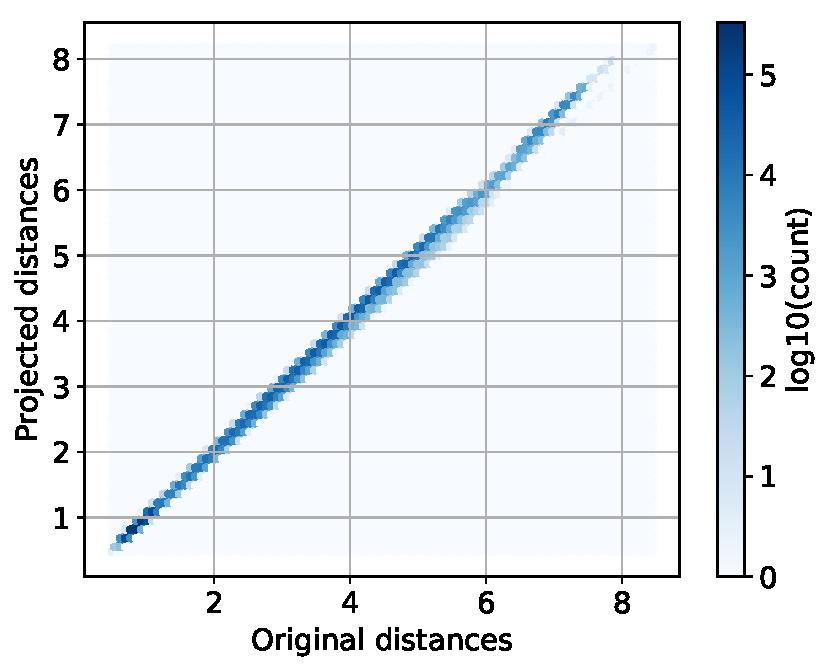
\includegraphics[width=\linewidth]{fig/streamhash_projection_euclidean_k1000.pdf}
				\caption{$K=1000$, Euclidean.}
		\end{subfigure}
    \caption{Distortion of streaming random projections for the Euclidean and cosine distance.}
		\label{fig:distortion}
\end{figure*}

\begin{figure*}[h!]
    \centering
    \begin{subfigure}[t]{0.29\textwidth}
        \centering
        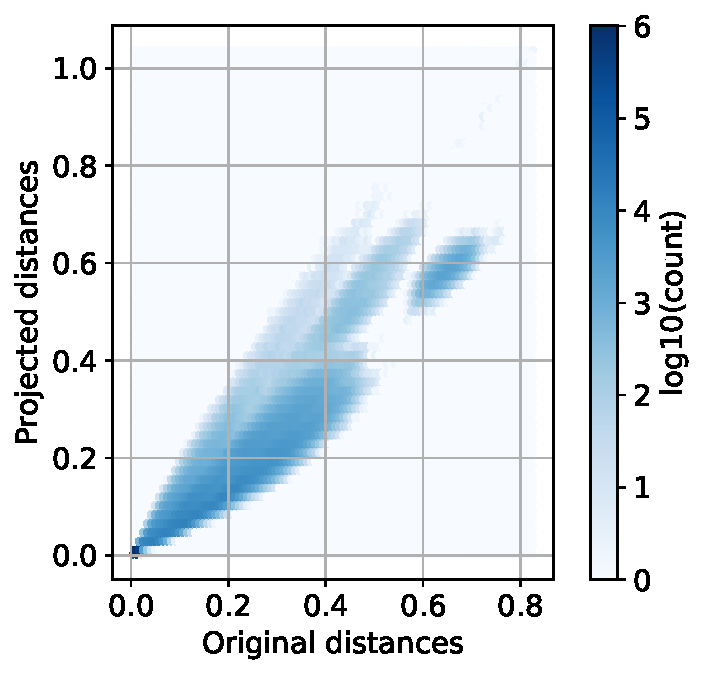
\includegraphics[width=\linewidth]{fig/sparse_projection_cosine_k50.pdf}
        \caption{$K=50$, cosine.}
    \end{subfigure}
    \hfill
		\begin{subfigure}[t]{0.29\textwidth}
				\centering
				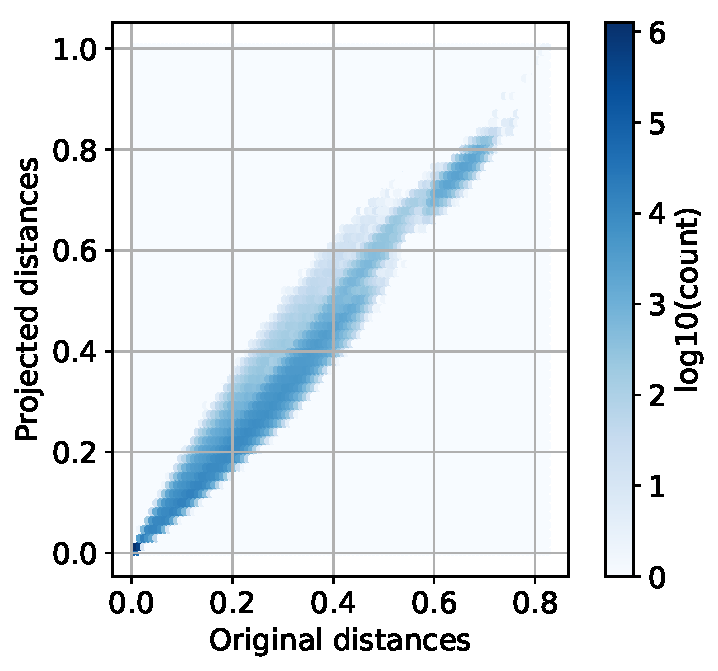
\includegraphics[width=\linewidth]{fig/sparse_projection_cosine_k100.pdf}
				\caption{$K=100$, cosine.}
		\end{subfigure}
		\hfill
		\begin{subfigure}[t]{0.29\textwidth}
				\centering
				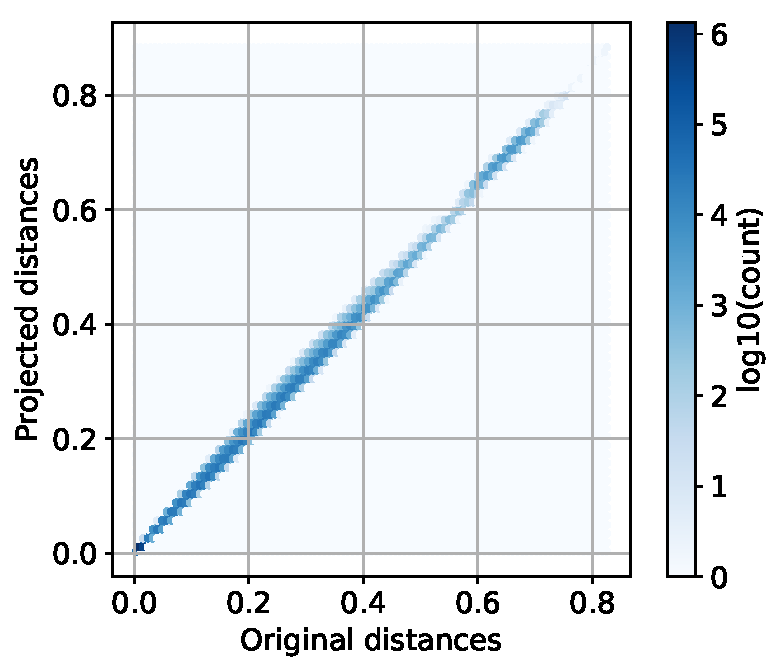
\includegraphics[width=\linewidth]{fig/sparse_projection_cosine_k1000.pdf}
				\caption{$K=1000$, cosine.}
		\end{subfigure}\\
		\begin{subfigure}[t]{0.29\textwidth}
				\centering
				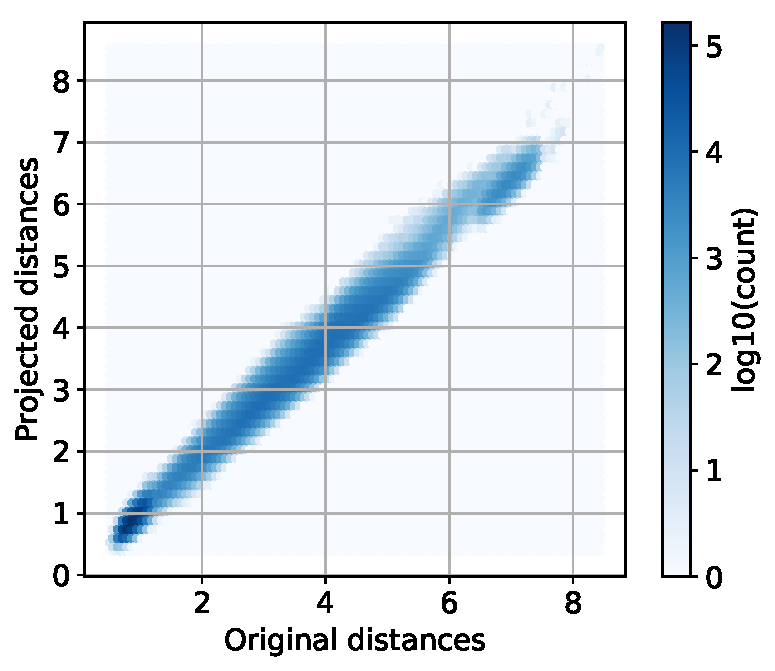
\includegraphics[width=\linewidth]{fig/sparse_projection_euclidean_k50.pdf}
				\caption{$K=50$, Euclidean.}
		\end{subfigure}
		\hfill
		\begin{subfigure}[t]{0.29\textwidth}
				\centering
				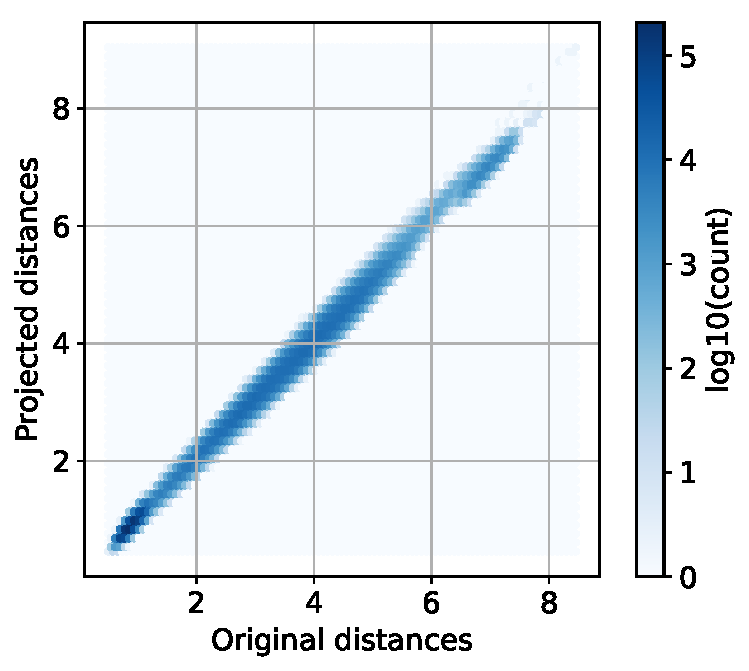
\includegraphics[width=\linewidth]{fig/sparse_projection_euclidean_k100.pdf}
				\caption{$K=100$, Euclidean.}
		\end{subfigure}
		\hfill
		\begin{subfigure}[t]{0.29\textwidth}
				\centering
				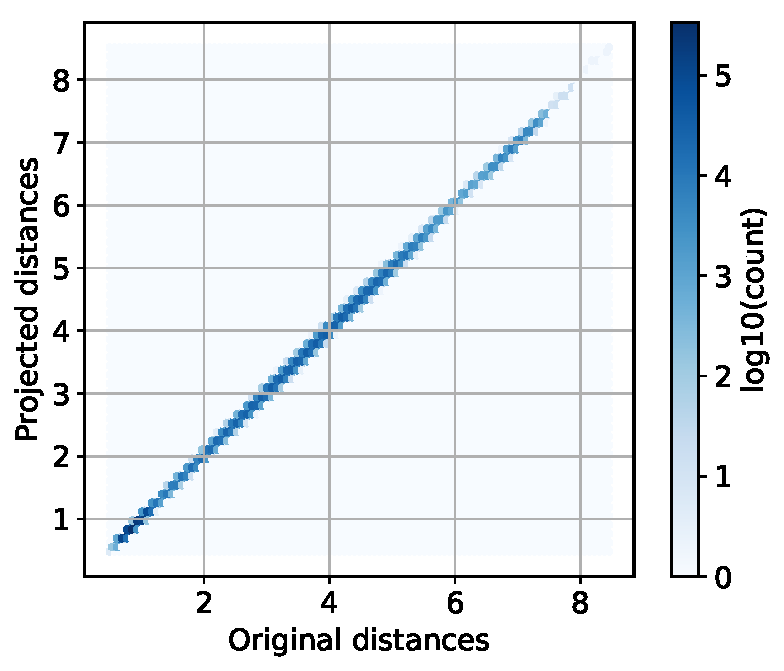
\includegraphics[width=\linewidth]{fig/sparse_projection_euclidean_k1000.pdf}
				\caption{$K=1000$, Euclidean.}
		\end{subfigure}
    \caption{Distortion for static random projections for the Euclidean and cosine distance.}
		\label{fig:distortion-static}
\end{figure*}

\pagebreak

\subsection{Addressing local density variation}

\begin{figure*}[ht!]
    \centering
		\begin{subfigure}[t]{0.3\textwidth}
				\centering
				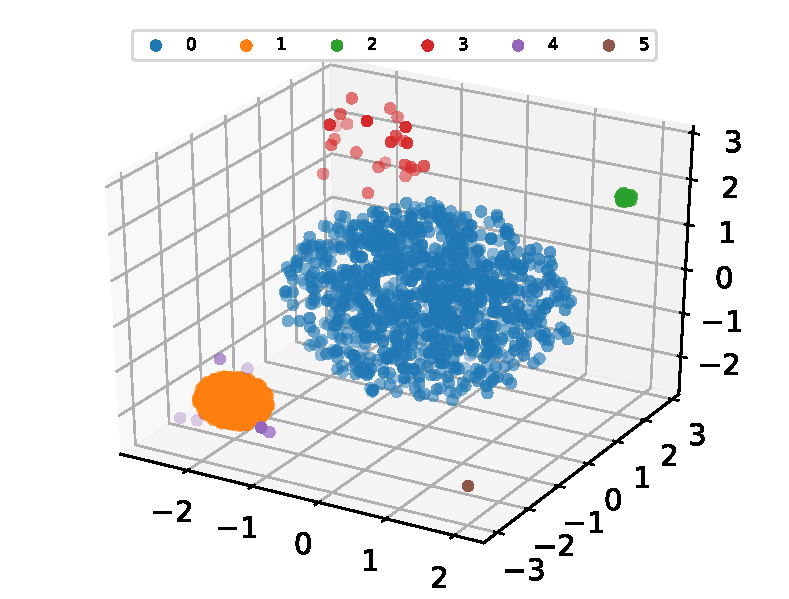
\includegraphics[width=\linewidth]{fig/syndata.pdf}
				\caption{Synthetic data.}
		\end{subfigure}
		\begin{subfigure}[t]{0.3\textwidth}
				\centering
				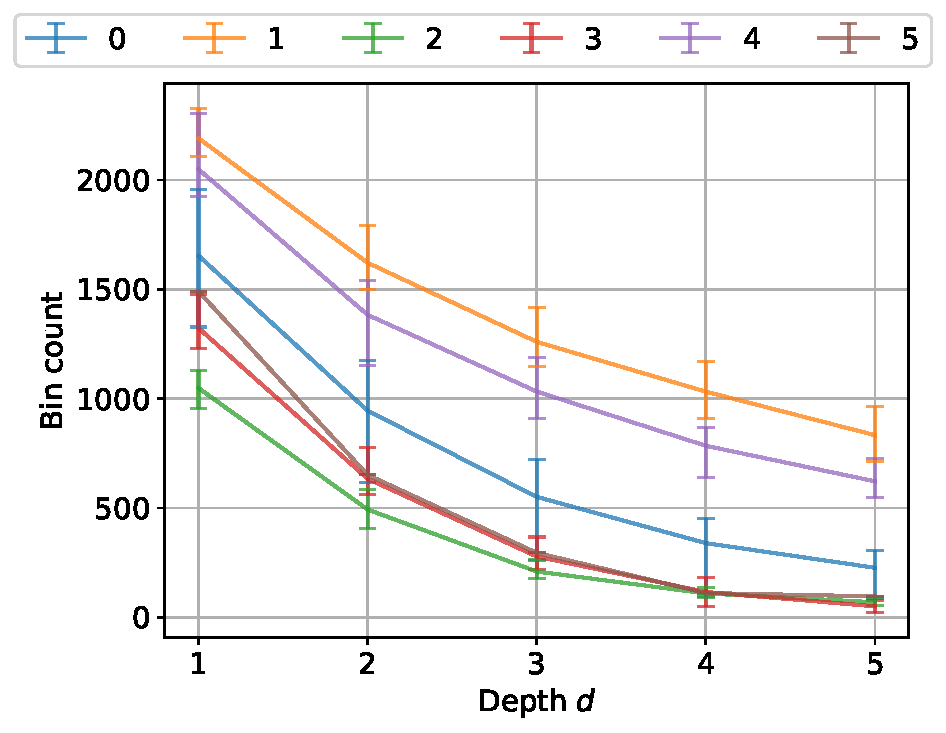
\includegraphics[width=\linewidth]{fig/chains_type_bincounts_k50c50d5.pdf}
				\caption{Bin-counts.}
		\end{subfigure}
		\hfill
    \begin{subfigure}[t]{0.3\textwidth}
        \centering
        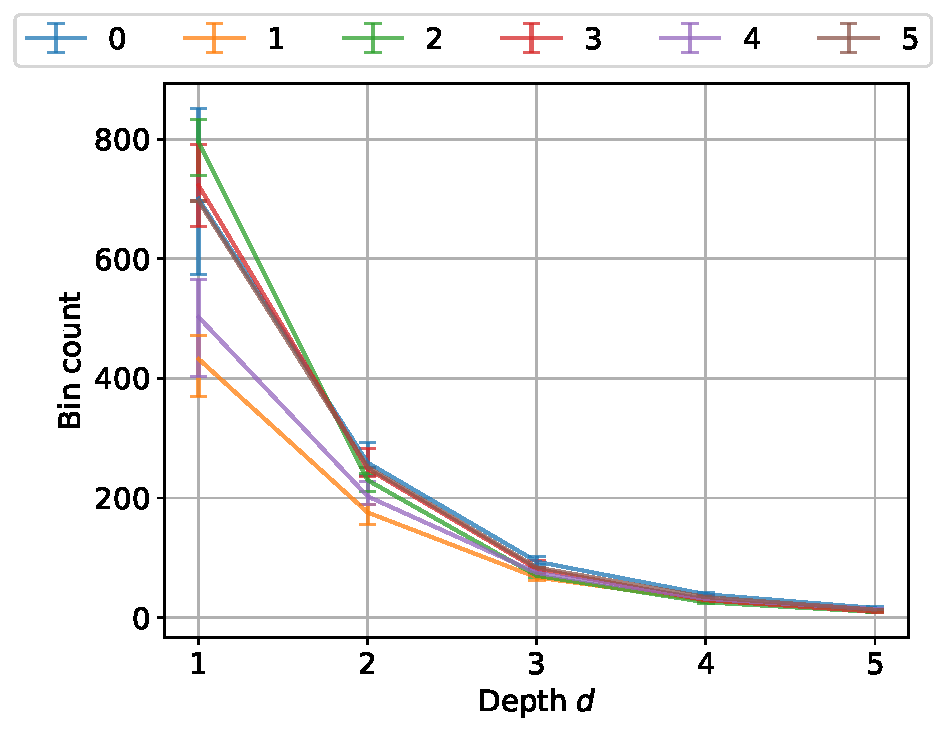
\includegraphics[width=\linewidth]{fig/chains_type_neighborbincounts_k50c50d5.pdf}
        \caption{Neighbor bin-counts.}
    \end{subfigure}\\
    \begin{subfigure}[t]{0.3\textwidth}
        \centering
        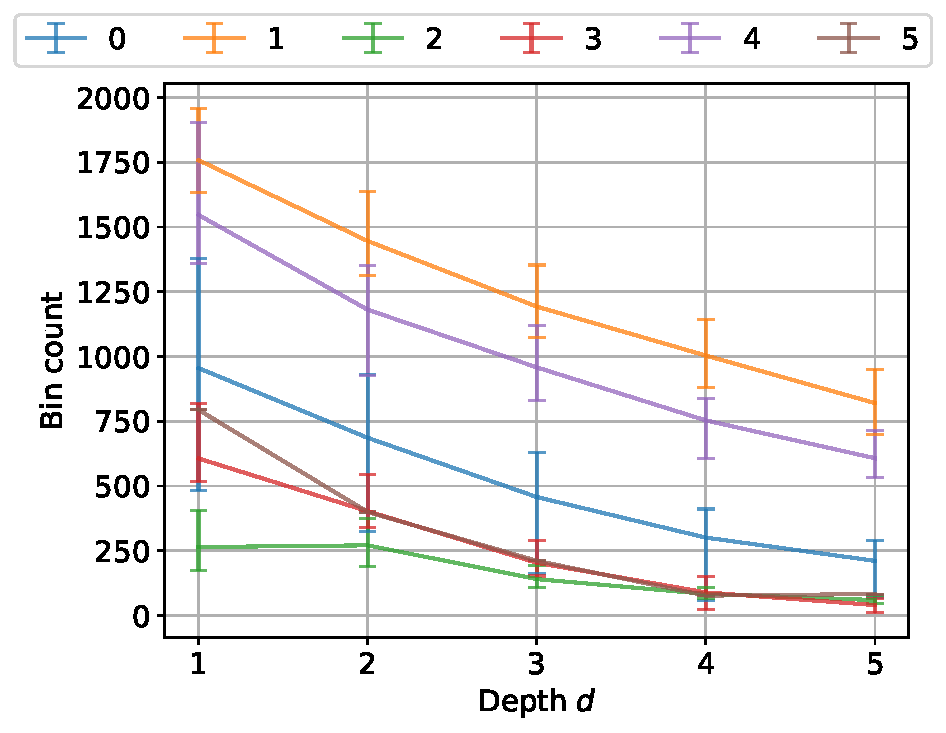
\includegraphics[width=\linewidth]{fig/chains_type_adjustedbincounts_k50c50d5.pdf}
        \caption{Adjusted bin-counts.}
    \end{subfigure}
		\hfill
    \begin{subfigure}[t]{0.3\textwidth}
        \centering
        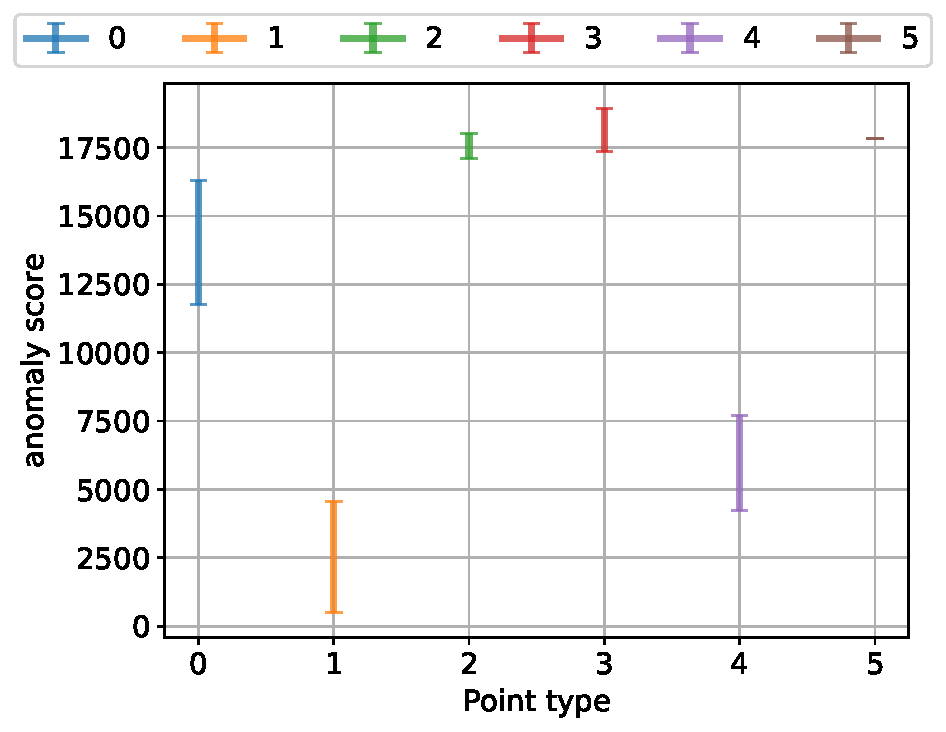
\includegraphics[width=\linewidth]{fig/chains_type_anomscores_k50c50d5.pdf}
        \caption{Anomaly scores.}
    \end{subfigure}
		\hfill
    \begin{subfigure}[t]{0.3\textwidth}
        \centering
        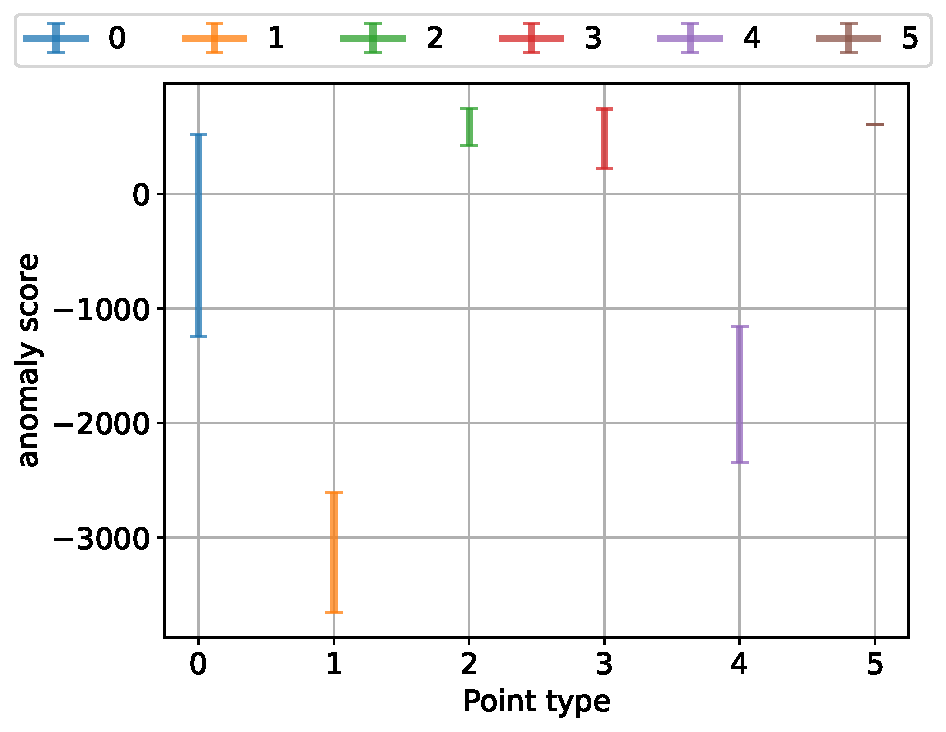
\includegraphics[width=\linewidth]{fig/chains_type_anomscores-adj_k50c50d5.pdf}
        \caption{Adjusted anomaly scores.}
    \end{subfigure}
    \caption{Score distributions for different point classes after addressing local density variation (see \S2.3 and \S2.7). Error bars indicate the median, 5$^{\textrm{th}}$ and 95$^{\textrm{th}}$ percentile scores across all points. Chains with $K=50, C=100, d=5$.}
\end{figure*}
\begin{wrapfigure}[12]{r}{0.25\textwidth}
    \centering
		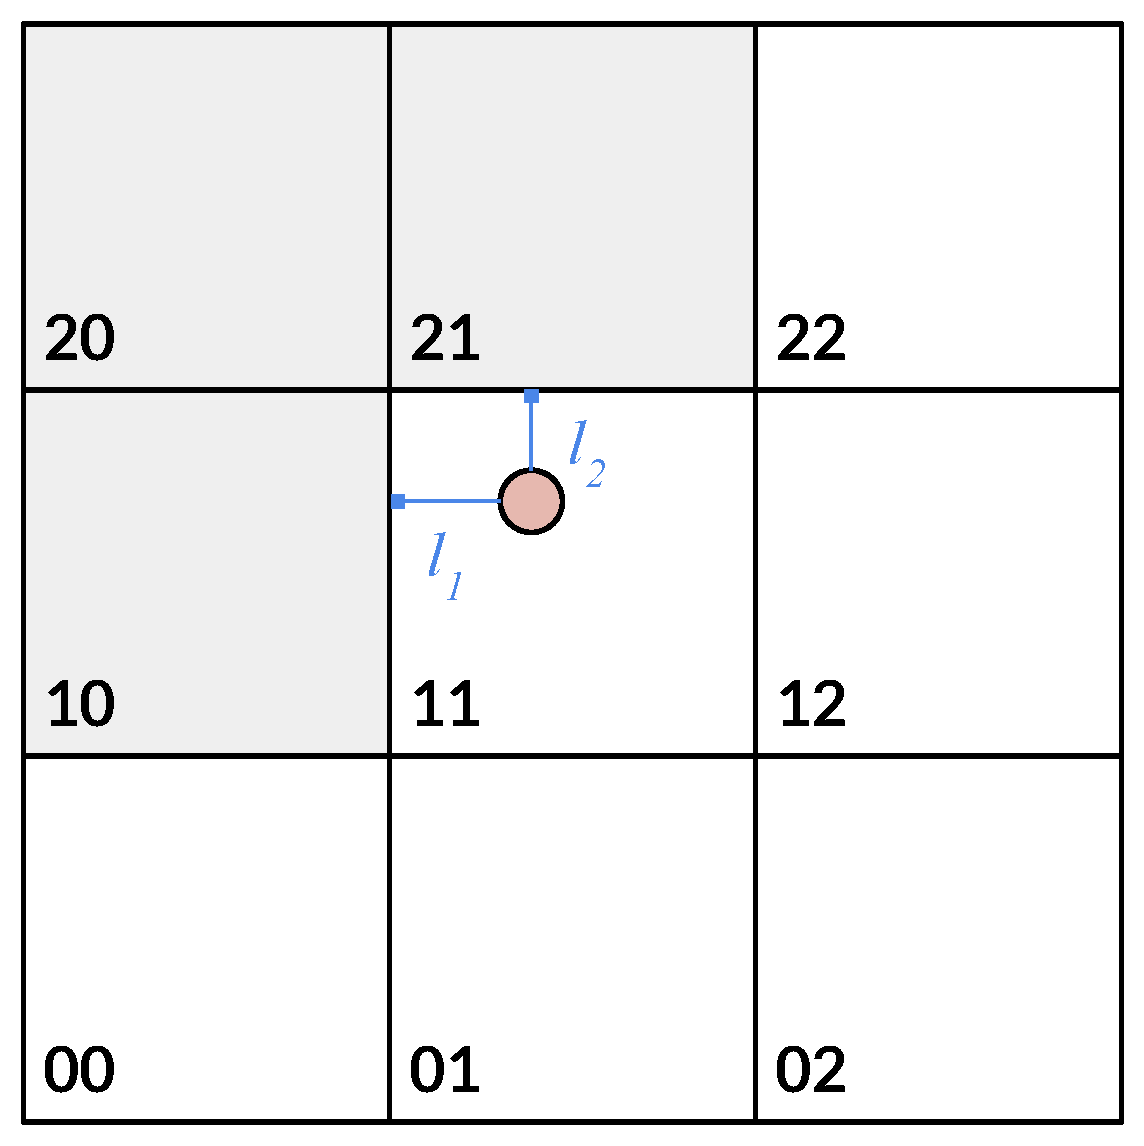
\includegraphics[width=\linewidth]{fig/grid.pdf}
    \caption{2-d grid.}
\end{wrapfigure}
Instead of adjusting the bin-count of each point $j$ with the mean bin-count of all other points, we could adjust it with the mean bin-count over \textit{neighboring bins}. This enables us to capture deviations in the \textit{local} density.

However, for a given point $j$ having a $d$-element bin-id at depth $d$, there are $3^d -1$ possible neighboring bins; enumerating all of them is infeasible, and most of them would be empty.

Instead, we could sample a fixed number of neighboring bins at random, such that the probability of sampling each neighboring bin is proportional to the likelihood of neighbors of $j$ lying in that bin This probability is proportional to the distance of the point $j$ to the edge of the neighboring bin (see $l_1$ and $l_2$ in Fig. 13: shaded neighboring bins are more likely to contain neighbors of the red point $j$). This idea was introduced as ``multi-probe LSH'' in \parencite{lv2007multi}.

Thus, for a point $j$ having a set of neighboring bins $\mathcal{N}(j)$, the adjusted LOCI score becomes:
\begin{eqnarray}
	L_{id}(\bar{Y}_j) &=& \bar{H}_{id}(\bar{Y}_j) - \frac{1}{|\mathcal{N}(j)|}\sum_{\bar{Y}_k \in \mathcal{N}(q)}\bar{H}_{id}(\bar{Y}_k)
\end{eqnarray}

\pagebreak

\subsection{Incremental maintenance of the LOCI score}

The LOCI score for chain $i$, point $j$ and depth $d$ was defined as:
\begin{eqnarray}
	L_{id}(\bar{Y}_j) &=& H_{id}(\bar{Y}_j)\times 2^d - \frac{1}{N}\sum_{k}H_{id}(\bar{Y}_k)\times 2^d
\end{eqnarray}
where $H_{id}(\bar{Y}_j)$ is the bin-count and is directly available on the arrival of every new point. Hence, the first term of the above equation is easily computable.

Let $b_{id}(c)$ be the bin-count of a bin $c$ in chain $i$ at depth $d$. Then the total bin-count $S_{id}$ (the sum of the bin-counts of all points in chain $i$ at depth $d$) is given by:
\begin{eqnarray}
	S_{id} = \sum_{k}H_{id}(\bar{Y}_k) = \sum_{c \in \textrm{bins in chain}(i,d)} b_{id}(c)^2
\end{eqnarray}
When a new point arrives, it falls into some cell $c'$, and its bin-count is incremented to $b_{id}(c') + 1$. This results in the following change to the total bin-count:
\begin{eqnarray}
	S'_{id} &=& \sum_{c \neq c'} b_{id}(c)^2 + (b_{id}(c') + 1)^2\\
					&=& \sum_{c} b_{id}(c)^2 + 2b_{id}(c') + 1\\
					&=& S_{id} + 2b_{id}(c') + 1
\end{eqnarray}
where $b_{id}(c)$ was the bin-count before the point was added, and is easily computable. This equation, along with tracking the number of points $N$, can thus be used to incrementally maintain the second term of the LOCI score.

\subsection{Dynamic chains with windows}

\pagebreak

\subsection{Streaming evaluation}

\begin{table}[ht!]
	\centering
	\begin{tabular}{llllll}
	\toprule
	\textbf{Dataset} & \textbf{Feature} & \textbf{Dynamic} & \textbf{Input size} 		  & \textbf{Dimensionality} & \textbf{Anomaly}\\
									 & \textbf{space}   & \textbf{updates} & \textbf{(incl. updates)} & \textbf{(maximum)} 			& \textbf{rate}\\
	\midrule
	network-intrusion& Fixed 	  		    & No				 & 720K    & 34   & 00.87\%\\
 	spam-sms 			 	 & Evolving 			  & No				 & 5574 	 & ? 	 & 14.00\%\\
 	spam-url 			 	 & Evolving 				& No				 & 3.2M    & 2.4M & 33.00\%\\
	streamspot-flash & Evolving 				& Yes				 & 111M    & ?    & 20.00\%\\
	streamspot-java  & Evolving 				& Yes				 & ?       & ?    & 20.00\%\\
	\bottomrule
	\end{tabular}
	\caption{Datasets used for the streaming evaluation.}
	\label{table:datasets}
\end{table}

\pagebreak

% !TEX root = ./xstream.tex

\section{Baselines}
\subsection{Datasets}
Datasets shown in Table~\ref{table:datasets}.

\begin{table}[]
\centering
\label{table:datasets}
\begin{tabular}{ccc}
\textbf{Dataset Name}         & \textbf{\#Samples} & \textbf{\#Features} \\	\hline \hline
breast-cancer-wisconsin (Mid) & 568                & 30                  \\
ionosphere (Mid)              & 350                & 33                  \\
magic-telescope (Low)         & 19020              & 10                  \\
pima-indians (Low)            & 768                & 8		\\
gisette (High) & 7000 & 4970	\\
isolet (High) & 7797 & 616		\\
letter-recognition (High) & 7797 & 616	\\
madelon (High) & 2600 & 500	\\
\end{tabular}
\caption{List of benchmark datasets used.}
\end{table}

\subsection{Adding Noise To Datasets}
We used $2$ different methods to generate benchmark datasets. The first method was applicable only to the low-dimensional and mid-dimensional datasets, and the second method was for high-dimensional datasets. We explain both of these methods below:
\textbf{Method 1}: We add noisy columns to the original dataset. The number of noisy columns is in the percentage of original number of columns that are added, and the noise level governs the mean and standard deviation of the gaussian distribution. We play around with percentage of noisy columns to be added, choosing values such as  100, 1000, 2000, and 5000. For noise-levels, we played with 0.01, 0.1, 0.2, 0.25. The mean and standard deviation of the Gaussian distribution was just noise-level multiplied with the original mean, or the original standard deviation of the entire dataset.

\textbf{Method 2}: We first discard all the original anomalous points. Now for the remaining nominal points, we first choose 10\% of the features and mark them as important features. We further proceed with choosing 5\% of the dataset as important samples. Now, in this sub-block, which contains only important samples and important features, we add Gaussian noise to the original data. Again, Gaussian noise is used, parameterized by the mean, and the standard deviation of the entire nominal dataset. Further this noise is scaled according to the user-specified signal to noise ratio, and added to the original sub-block of our dataset and features.

\subsection{Baseline Algorithms}
\begin{itemize}
\item{\textbf{iForest}: We use it with recommended sample size of $256$ or the entire dataset, whichever is minimum. The hlim is set to $15$ to be comparable to HS-Trees, and number of components is set to $100$.}
\item{\textbf{HS-Trees}:  Use it with recommended setting of $15$ max depth trees, and number of components is $100$.}
\item{\textbf{LODA}: We set the sparsity factor to $\frac{1}{\sqrt(d)}$. We allow LODA to select best width for histograms, but fix the number of histograms to $100$ to be comparable to rest of the algorithms.}
\item{\textbf{RS-Hash}: For RS-Hash, we use $1000$ sampling points, as recommended and $100$ components.}
\end{itemize}

\subsection{Baseline Results}
\begin{footnotesize}
\begin{table}[ht!]
    \centering
		\begin{tabular}{lllllll}
				\toprule
				\textbf{Dataset} & \textbf{IF} &  \textbf{LODA} & \textbf{RSH} &  \textbf{HST}  & \textbf{XS}\\
				\midrule
				\multicolumn{3}{c}{\textit{High-dimensional Datasets}}\\
%gisette& $0.423 \pm 0.011$ &  $0.436 \pm 0.008$ &  $0.417 \pm 0.005$ &  $0.432 \pm 0.017$    \\
gisette (30,0.3,1.2)& $0.683 \pm 0.045$ &  $0.531 \pm 0.018$ &  $0.46 \pm 0.005$ &  $0.628 \pm 0.021$    \\
gisette (30,0.3,10)& $0.541 \pm 0.027$ &  $0.321 \pm 0.004$ &  $0.354 \pm 0.002$ &  $0.471 \pm 0.024$    \\
gisette (30,0.3,20)& $0.45 \pm 0.022$ &  $0.29 \pm 0.003$ &  $0.308 \pm 0.003$ &  $0.347 \pm 0.017$    \\
gisette (30,0.3,30)& $0.432 \pm 0.016$ &  $0.301 \pm 0.005$ &  $0.31 \pm 0.002$ &  $0.316 \pm 0.006$    \\
\midrule
%isolet& $0.442 \pm 0.019$ &  $0.429 \pm 0.02$ &  $0.444 \pm 0.001$ &  $0.444 \pm 0.013$    \\
isolet (30.0,0.3,1.2)& $0.537 \pm 0.03$ &  $0.58 \pm 0.03$ &  $0.441 \pm 0.01$ &  $0.559 \pm 0.028$    \\
isolet (30.0,0.3,10)& $0.372 \pm 0.011$ &  $0.35 \pm 0.007$ &  $0.334 \pm 0.004$ &  $0.391 \pm 0.015$    \\
isolet (30.0,0.3,20)& $0.33 \pm 0.009$ &  $0.313 \pm 0.006$ &  $0.311 \pm 0.001$ &  $0.322 \pm 0.007$    \\
isolet (30.0,0.3,30)& $0.3 \pm 0.002$ &  $0.292 \pm 0.004$ &  $0.296 \pm 0.001$ &  $0.293 \pm 0.002$    \\
\midrule
%letter-recognition& $0.475 \pm 0.012$ &  $0.46 \pm 0.011$ &  $0.453 \pm 0.003$ &  $0.471 \pm 0.009$    \\
letter-recognition (30.0,0.3,1.2)& $0.49 \pm 0.026$ &  $0.534 \pm 0.03$ &  $0.44 \pm 0.01$ &  $0.519 \pm 0.053$    \\
letter-recognition (30.0,0.3,10)& $0.374 \pm 0.015$ &  $0.337 \pm 0.003$ &  $0.339 \pm 0.008$ &  $0.375 \pm 0.007$    \\
letter-recognition (30.0,0.3,20)& $0.309 \pm 0.008$ &  $0.289 \pm 0.002$ &  $0.291 \pm 0.002$ &  $0.31 \pm 0.007$    \\
letter-recognition (30.0,0.3,30)& $0.319 \pm 0.01$ &  $0.305 \pm 0.003$ &  $0.308 \pm 0.001$ &  $0.307 \pm 0.004$    \\
\midrule
%madelon& $0.501 \pm 0.008$ &  $0.515 \pm 0.014$ &  $0.507 \pm 0.003$ &  $0.511 \pm 0.01$    \\
madelon (5.0,0.05,1.2)& $0.896 \pm 0.051$ &  $1.0 \pm 0.0$ &  $0.92 \pm 0.007$ &  $0.969 \pm 0.039$    \\
madelon (5.0,0.05,10)& $0.643 \pm 0.13$ &  $0.988 \pm 0.012$ &  $0.784 \pm 0.068$ &  $0.899 \pm 0.094$    \\
madelon (5.0,0.05,20)& $0.24 \pm 0.093$ &  $0.112 \pm 0.027$ &  $0.16 \pm 0.039$ &  $0.377 \pm 0.143$    \\
madelon (5.0,0.05,30)& $0.07 \pm 0.013$ &  $0.054 \pm 0.007$ &  $0.083 \pm 0.004$ &  $0.099 \pm 0.059$    \\

				\bottomrule
		\end{tabular}
		\caption{AP for Baseline algorithms on High Dimensional Dataset. The numbers in bracket indicates the percentage of features, fraction of samples to which noise is added, and the SnR ratio of noise respectively.}
\end{table}
\end{footnotesize}

\begin{footnotesize}
\begin{table}[ht!]
    \centering
		\begin{tabular}{llllll}
				\toprule
				\textbf{Dataset} & \textbf{IF} & \textbf{LODA} & \textbf{RSH} & \textbf{HST} & \textbf{XS}	\\
				\midrule
				\multicolumn{3}{c}{\textit{Low/medium-dimensional Datasets}}\\
breast-cancer& $0.635 \pm 0.024$ &  $0.883 \pm 0.019$ &  $0.758 \pm 0.004$ &  $0.719 \pm 0.019$    \\
breast-cancer (100,0.1)& $0.661 \pm 0.036$ &  $0.839 \pm 0.024$ &  $0.727 \pm 0.01$ &  $0.702 \pm 0.026$    \\
breast-cancern (1000,0.1)& $0.476 \pm 0.043$ &  $0.686 \pm 0.047$ &  $0.394 \pm 0.007$ &  $0.531 \pm 0.047$    \\
breast-cancer (2000,0.1)& $0.447 \pm 0.026$ &  $0.643 \pm 0.066$ &  $0.444 \pm 0.015$ &  $0.474 \pm 0.046$    \\
breast-cancer (5000,0.1)& $0.404 \pm 0.021$ &  $0.508 \pm 0.086$ &  $0.4 \pm 0.013$ &  $0.425 \pm 0.022$    \\
\midrule
ionosphere& $0.819 \pm 0.008$ &  $0.79 \pm 0.014$ &  $0.824 \pm 0.003$ &  $0.83 \pm 0.005$    \\
ionosphere (100,0.1)& $0.756 \pm 0.031$ &  $0.771 \pm 0.013$ &  $0.773 \pm 0.005$ &  $0.725 \pm 0.018$    \\
ionosphere (1000,0.1)& $0.59 \pm 0.044$ &  $0.742 \pm 0.032$ &  $0.573 \pm 0.008$ &  $0.579 \pm 0.054$    \\
ionosphere (2000,0.1)& $0.441 \pm 0.033$ &  $0.736 \pm 0.029$ &  $0.505 \pm 0.033$ &  $0.446 \pm 0.027$    \\
ionosphere (5000,0.1)& $0.403 \pm 0.022$ &  $0.675 \pm 0.048$ &  $0.376 \pm 0.006$ &  $0.399 \pm 0.028$    \\
\midrule
magic-telescope& $0.655 \pm 0.011$ &  $0.623 \pm 0.004$ &  $0.674 \pm 0.003$ &  $0.678 \pm 0.005$    \\
magic-telescope (100,0.1)& $0.593 \pm 0.01$ &  $0.617 \pm 0.003$ &  $0.576 \pm 0.005$ &  $0.601 \pm 0.015$    \\
magic-telescope (1000,0.1)& $0.451 \pm 0.018$ &  $0.592 \pm 0.013$ &  $0.419 \pm 0.008$ &  $0.471 \pm 0.021$    \\
magic-telescope (2000,0.1)& $0.407 \pm 0.021$ &  $0.586 \pm 0.007$ &  $0.407 \pm 0.003$ &  $0.409 \pm 0.018$    \\
magic-telescope (5000,0.1)& $0.376 \pm 0.011$ &  $0.538 \pm 0.026$ &  $0.38 \pm 0.002$ &  $0.378 \pm 0.005$    \\
\midrule
pima-indians& $0.498 \pm 0.015$ &  $0.48 \pm 0.015$ &  $0.502 \pm 0.005$ &  $0.518 \pm 0.006$    \\
pima-indians (100,0.1)& $0.477 \pm 0.013$ &  $0.472 \pm 0.01$ &  $0.444 \pm 0.009$ &  $0.478 \pm 0.007$    \\
pima-indians (1000,0.1)& $0.385 \pm 0.017$ &  $0.444 \pm 0.014$ &  $0.379 \pm 0.006$ &  $0.397 \pm 0.024$    \\
pima-indians (2000,0.1)& $0.35 \pm 0.014$ &  $0.41 \pm 0.016$ &  $0.361 \pm 0.005$ &  $0.369 \pm 0.023$    \\
pima-indians (5000,0.1)& $0.343 \pm 0.008$ &  $0.4 \pm 0.028$ &  $0.338 \pm 0.003$ &  $0.349 \pm 0.014$    \\
				\bottomrule
		\end{tabular}
		\caption{AP over 10 runs for Low Dimensional Datasets. The numbers in the brackets alongside the dataset name indicate the percentage of original columns, added as noise, and the relative noise factor, respectively.}
\end{table}
\end{footnotesize}


\begin{table}[]
\centering
\begin{tabular}{l|lll}
\hline	\hline
\textbf{Friedman Statistic} & \textbf{Low-Dim Datasets} & \textbf{High-Dim Datasets} & \textbf{All Datasets}    \\ \hline
p-value            & 1.155e-09        & 8.362e-10         & \textless2.2e-16 \\ \hline \hline
\textbf{Wilcoxon Test}      & \multicolumn{3}{c}{\textbf{p-val w/ XST}}                        \\ 	\hline
iFor               & 1.907e-06         & 0.7271         &  0.001196       \\
RSH                & 6.676e-06         & 0.7392         & 0.002026        \\
LODA               & 9.537e-07         & 0.1744         & 0.0001096            \\
HSTrees            & 2.861e-06        & 0.2375          &  2.049e-05	\\	\hline
\end{tabular}
\caption{Friedman's test statistics among methods. And wilcoxon test p-values, indicating that XStream performs better than all the baseline methods for low-dimensional datasets and over the set of all datasets, but no method is more significant than XStream and vice-versa.}
\label{my-label}
\end{table}

\subsection{Time and Space Complexity}
%
%

\begin{table}[ht!]
	\caption{Symbol List}
	\centering
	\begin{tabular}{lll}
		\toprule
		\textbf{Symbols} & \textbf{Description}	\\	\hline
		$N$ & Number of data points	\\	\hline
		$D$ & Number of dimensions/features	\\	\hline
		$C$ & Number of ensemble components (trees, chains, histograms, etc.)	\\	\hline
		$d$ & Max depth of trees/chains	\\	\hline
		$\psi$ & iForest/HS-Trees/RS-Hash: sampling size	\\	\hline
		$r$ & RS-Hash: Number of sampled dimensions	\\
		$b$ & LODA: number of histogram bins	\\	\hline
		$m$ & \method/RS-Hash: Number of CMS hash functions	\\
		$L$ & \method/RS-Hash:: CMS hash table size	\\	\hline
		$k$ & \method: Number of random projections	\\
		$M$ & \method: Number of subspaces	\\
		$W$ & \method: Number of windows	\\
		\bottomrule
	\end{tabular}

\end{table}

\begin{table}[ht!]
	\caption{Time and space complexity of the ensemble anomaly detection algorithms compared in this paper.
		In streaming case, a data point/vector arrives at a time for HS-Stream, LODA, and RS-Hash; whereas
		an update to a single feature for a data point arrives at a time.}

	\centering
	\begin{tabular}{l|lclcl}
		\toprule
		\textbf{Algorithm} & \multicolumn{2}{l}{\textbf{Time Complexity}} &&& \textbf{Space Complexity}	\\
		& \multicolumn{3}{l}{\noindent\rule[0.5ex]{0.5\linewidth}{1pt}}
		& &  \multicolumn{1}{l}{\noindent\rule[0.5ex]{0.2\linewidth}{1pt}} \\
		& Training && Scoring/Updating && \\\hline
		{\em Batch/Offline} &&& & & \\
		iForest & $O(C\psi \log \psi)$ & & $O(C \log \psi)$ &  & $O(C\psi)$	\\
		HS-Trees & $O(Cd\psi)$ & &$O(Cd)$ && $O(C2^d)$ \\
		LODA & $O(NC\sqrt{D})$  & & $O(C\sqrt{D})$  && $O(C\sqrt{D} + Cb)$ \\
		RS-Hash & $O(Crm\psi)$ & & $O(Crm)$ && $O(CLm)$\\
		\method & $O(M[NDk + Ckmd])$ & &$O(M[Dk + Ckmd])$ && $O(MCLmd)$   \\
		\hline
		{\em Streaming/Online}  & & &&& \\
		HS-Stream & \multicolumn{1}{c}{--} & & $O(Cd + C\psi)$ && $O(C2^d)$ \\
		LODA & \multicolumn{1}{c}{--} & &$O(C\sqrt{D} + Cb)$ && $O(C\sqrt{D} + Cb)$\\
		RS-Hash & \multicolumn{1}{c}{--} & & $O(Crm)$ && $O(CLm)$\\
		\method & \multicolumn{1}{c}{--} & & $O(WMCkmd)$  && $O(WMCLmd)$   \\
		\bottomrule
	\end{tabular}
\end{table}

\subsection{Results}
\textbf{AUC / AP Results}



\textbf{Time-Analysis}
iForest is the fastest, RSHash is the slowest (RSHash implementation, however can be optimized)
\begin{figure*}[ht!]
    \centering
    \begin{subfigure}[t]{0.48\textwidth}
        \centering
        \includegraphics[width=\linewidth]{fig/baseline/TimeAnalysis_LowDim.png}
        \caption{Low/Mid - dimensional dataset analysis}
    \end{subfigure}
    \hfill
    \begin{subfigure}[t]{0.48\textwidth}
        \centering
        \includegraphics[width=\linewidth]{fig/baseline/TimeAnalysis_HighDim.pdf}
        \caption{High dimensional dataset analysis}
    \end{subfigure}
		\hfill
    \caption{RunTimes of algorithms over datasets with different noise levels. X-axis is over different datasets with different noise levels. Y-axis is log of runtime (in seconds).}
\end{figure*}

\subsection{Streaming Baseline Setup}

\textbf{Datasets}:

We use the same datasets as in HighDimension case in static setting. We create $10$ shuffled versions for each dataset. The datasets could either be shuffled randomly or it could be clustered in time. For the clustered shuffled, the input also includes a clustering percentage, that is how much percentage of anomalies should be clustered in time. We currently do not experiment with clustered in time datasets.

\textbf{Algorithms}
\begin{itemize}
\item{RS-Hash}: We use decay constant to be $0.015$, and use first $256$ samples to setup the $100$ components, and then compute AUC/AP over time.
\item{HS-Trees}:
\item{LODA}:
\end{itemize}

\textbf{Results}

\begin{figure*}[ht!]
    \centering
    \begin{subfigure}[t]{0.48\textwidth}
        \centering
        \includegraphics[width=\linewidth]{fig/streaming_baseline/letter-recognition.pdf}
        \caption{Low/Mid - dimensional dataset analysis}
    \end{subfigure}
    \hfill
    \begin{subfigure}[t]{0.48\textwidth}
        \centering
        \includegraphics[width=\linewidth]{fig/streaming_baseline/madelon.pdf}
        \caption{High dimensional dataset analysis}
    \end{subfigure}
		\hfill
    \caption{AP for two of the baseline datasets over time, using RS-Hash Streaming Algorithm.}
\end{figure*}

% Using the median instead of the mean in eq. (6) improves performance slightly.
%
% \begin{table}[h!]
% 	\centering
% 	\begin{tabular}{lll}
% 		\toprule
% 		\textbf{Chain Parameters} & \textbf{Mean AP} & \textbf{Standard Deviation}\\
% 		\midrule
% 		$K=50, C=10$ & 0.830 & 0.096\\
% 		$K=50, C=50$ & 0.930 & 0.003\\
% 		$K=25, C=10$ & 0.804 & 0.076\\
% 		$K=25, C=50$ & 0.903 & 0.010\\
% 		\bottomrule
% 	\end{tabular}
% 	\caption{Chain AP stability across 5 runs, median instead of mean in eq. (6), $D=10$.}
% \end{table}

\pagebreak


% !TEX root = ./xstream.tex

\section{Dynamic evaluation}

\textbf{Datasets}:

We use the same datasets as in HighDimension case in static setting. We create $10$ shuffled versions for each dataset. The datasets could either be shuffled randomly or it could be clustered in time. For the clustered shuffled, the input also includes a clustering percentage, that is how much percentage of anomalies should be clustered in time. We currently do not experiment with clustered in time datasets.

\textbf{Algorithms}
\begin{itemize}
\item{RS-Hash}: We use decay constant to be $0.015$, and use first $256$ samples to setup the $100$ components, and then compute AUC/AP over time.
\item{HS-Trees}:
\item{LODA}:
\end{itemize}

\textbf{Results}

\begin{figure*}[ht!]
    \centering
    \begin{subfigure}[t]{0.48\textwidth}
        \centering
        \includegraphics[width=\linewidth]{fig/streaming_baseline/letter-recognition.pdf}
        \caption{Low/Mid - dimensional dataset analysis}
    \end{subfigure}
    \hfill
    \begin{subfigure}[t]{0.48\textwidth}
        \centering
        \includegraphics[width=\linewidth]{fig/streaming_baseline/madelon.pdf}
        \caption{High dimensional dataset analysis}
    \end{subfigure}
		\hfill
    \caption{AP for two of the baseline datasets over time, using RS-Hash Streaming Algorithm.}
\end{figure*}

\pagebreak


\printbibliography
\end{document}
